%!TEX root = ../thesis.tex
\externaldocument[A-]{Chapters/appendix.tex}

\part{Muxmon experiment}

  \textbf{large TODO:}
  \begin{itemize}
    \item Explain surface code architecture
    \item Explain the general structure of a chip:
    \begin{itemize}
      \item Feedline through which signal is sent and measured
      \item CPW resonators, capacitively coupled to feedline
      \item Single qubit coupled to resonators (coupling location?)
      \item Resonator buses
    \end{itemize}
    \item Explain multiplexed readout
  \end{itemize}

  \textbf{small TODO:}
  \begin{itemize}
    \item Rename DAC voltage to flux, and mention early on that this renaming will be used
    \item flux-bias line or flux bias line?
  \end{itemize}



  \chapter*{Introduction}

    At this moment circuit QED is at the stage where multi-qubit experiments are being realized.

    \begin{itemize}
        \item Scaling up
        \item Challenges involved in scaling
        \item Frequency re-use, Duplexer intro
    \end{itemize}


  \chapter{Challenges in scaling up}
    \label{ch:Muxmon chip architecture}

    \section{frequency re-use}
      \begin{wrapfigure}[16]{r}{0.45\textwidth}
        \begin{center}
        \vspace{-30pt}
          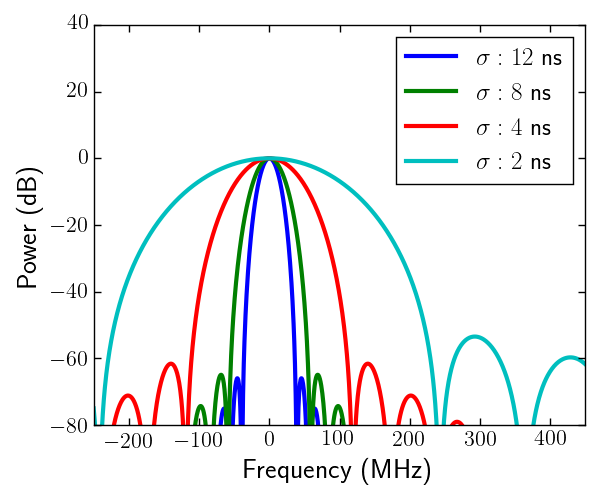
\includegraphics[width=\textwidth]{../Figures/Exploring frequency re-use/bandwidth_broadening.png}
        \end{center}
        \caption{The frequency bandwidth corresponding to Gaussian pulses with different widths $\sigma$.}
        \label{fig:bandwidth broadening}
        \vspace{-20pt}
      \end{wrapfigure}

      Even in large-scale quantum circuits individual qubit control is required. When multiple qubits are connected to a single drive line, being able to control the qubits individually requires their frequencies to be sufficiently separated. The amount by which the frequencies must be separated depends on the length of the pulses applied to the qubit. The shorter the pulse, the larger its corresponding frequency bandwidth, as can be seen in Figure~\ref{fig:bandwidth broadening}. Longer pulses, on the other hand, result in less operations being possible within the coherence times of the qubit. It is therefore desirable to have pulses with a short duration. This means that the separation between qubit frequencies must be large. Since there is only a finite frequency spectrum, having many qubits, each with a different frequency, results in frequency crowding.

      If the qubits are not connected to the same drive line, they can be individually controlled, even when they share the same frequency. This concept is known as frequency re-use, and is a possible way to overcome frequency crowding. Frequency re-use can be implemented in the surface code architecture. One possible implementation of frequency re-use in the surface code is shown in Figure~\ref{fig:surface code frequency re-use}, where every resonator is connected to four qubits. In this set-up four distinct frequencies suffice to enable individual driving of every qubit on the lattice.

      \begin{figure}[h]
        \centering
        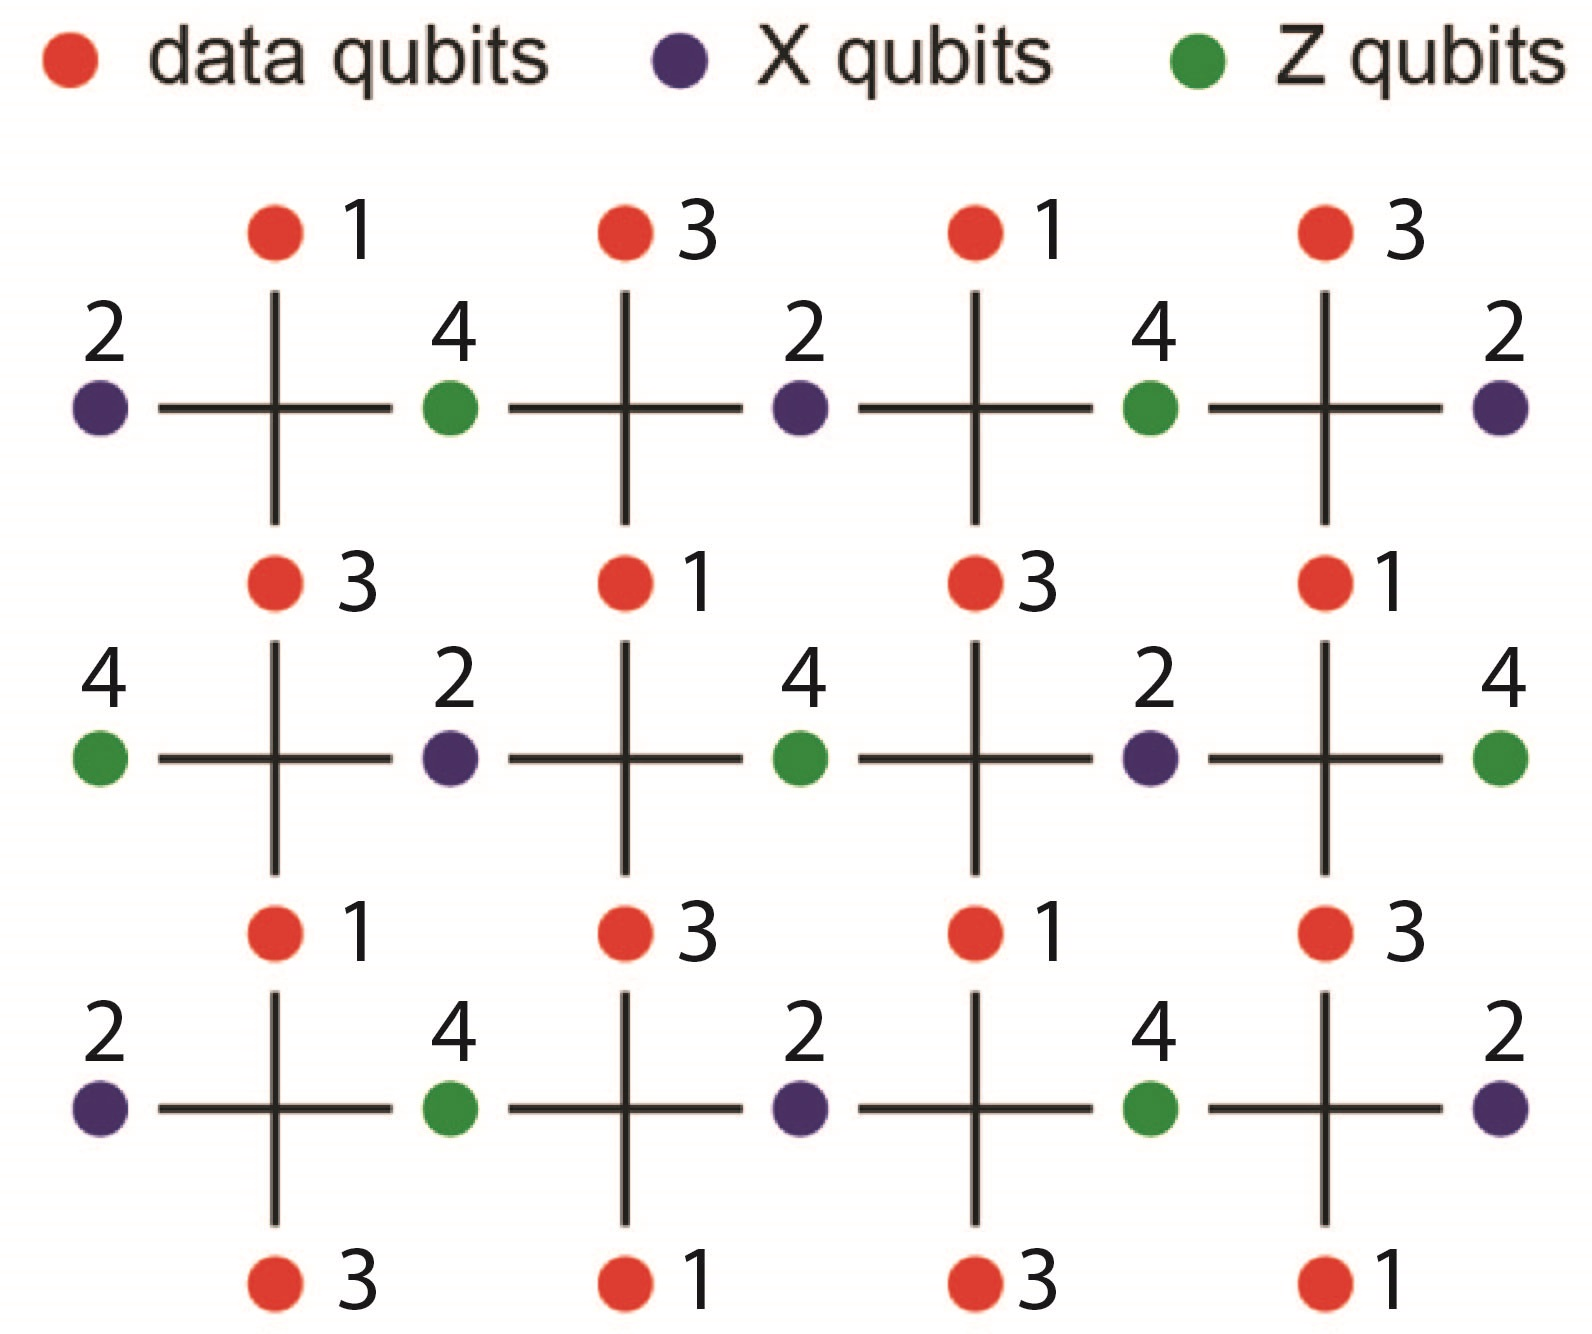
\includegraphics[width=.6\textwidth]{../Figures/Exploring frequency re-use/surface_code_frequency re-use_cut.jpg}
        \caption{A surface code architecture with the implementation of frequency re-use. The different digits correspond to distinct frequencies. }
        \label{fig:surface code frequency re-use}
      \end{figure}

      Frequency re-use does pose potential issues. Two unwanted effects in particular arise when multiple qubits that are directly or indirectly coupled to each other share the same frequency. The first effect is cross-coupling, where an excitation can be transferred from one qubit to the other. This will be discussed in Section~\ref{sec:cross-coupling}. The second effect is cross-driving, where a pulse that partially leaks through the components will drive other qubits. The components separating qubits do not act as perfect filters, and so the pulse will always partially leak through. This does not pose a problem as long as the frequency of the pulse is sufficiently detuned from the frequency of the other qubits. In the case of frequency re-use, however, the frequencies of the qubits are the same, and so a pulse leaking through will result in cross-driving. This effect is discussed in Section~\ref{sec:cross-driving}.

    \section{Selective broadcasting}
      \label{sec:selective broadcasting using the Duplexer}
      \begin{wrapfigure}[13]{r}{0.45\textwidth}
        \begin{center}
        \vspace{-30pt}
          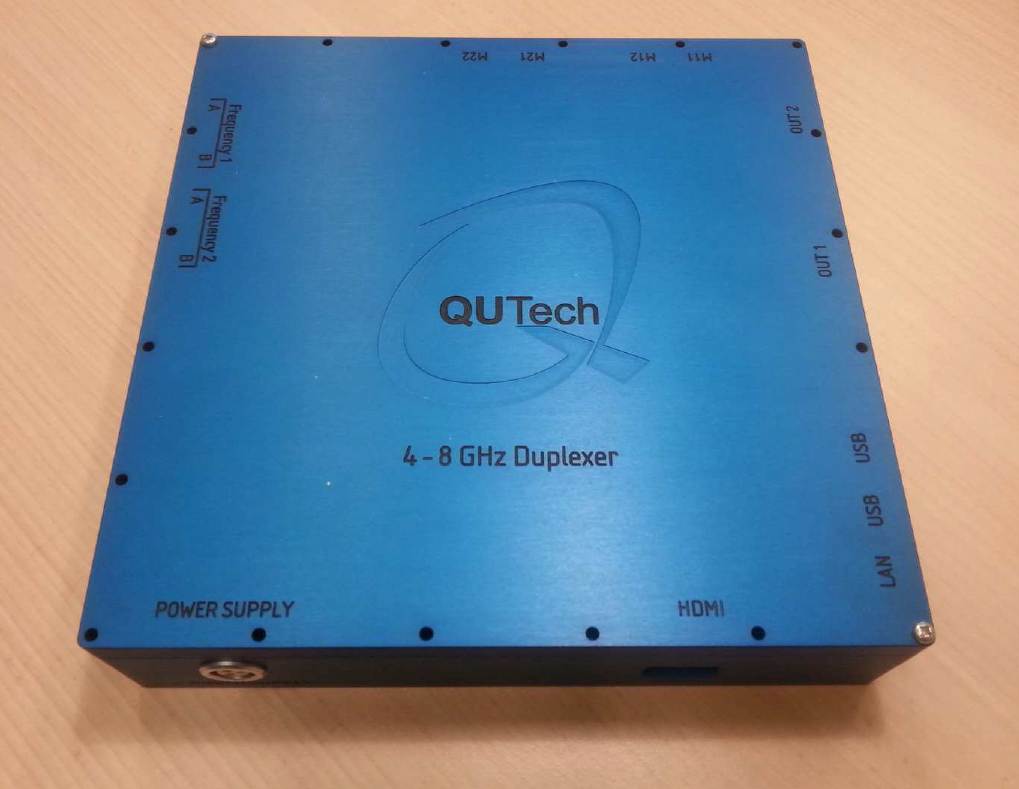
\includegraphics[width=\textwidth]{../Figures/Duplexer_with_background.png}
        \end{center}
        \vspace{-5pt}
        \caption{The Duplexer}
        \label{fig:Duplexer picture}
        \vspace{-10pt}
      \end{wrapfigure}

      A second challenge that exists when scaling up is that as the number of qubits grow, so do the instruments needed to control them. When thinking of a large-scale quantum computer, it is unrealistic to think that each qubit will have its own RF generator, AWG, and other necessary instruments. Therefore, alternatives have to be devised to combat this scaling of instruments. One such device is the Duplexer, shown in Figure~\ref{fig:Duplexer picture}. The Duplexer is a patented vector switch matrix designed by Duije Deurloo, who is working at TNO. It has four input ports and two ouput ports. Signals going through each of the input-output port combinations pass through the following successive components:

      \begin{enumerate}
        \item Digital switch
        \item Variable phase-shifter
        \item Variable attenuator
        \item Amplifier
      \end{enumerate}

      The Duplexer's digital switches have an RF-switching time of \SI{4}{\nano \second}. Using these switches, pulses may be sent to either of the two output ports, or to both output ports simultaneously. This allows for selective broadcasting, where pulses are routed to either or both of the two output ports at the nanosecond scale. When the output ports are connected to drive lines that are connected to qubits sharing the same frequency, the result is that two qubits can be controlled using a single generator and AWG. This property will be exploited in Randomized Benchmarking in Chapter~\ref{ch:randomized benchmarking}.

    \section{The Muxmon experiment}
      \label{sec: the Muxmon experiment}
      \begin{figure}[h]
      \centering
        \begin{subfigure}[b]{0.9\textwidth}
          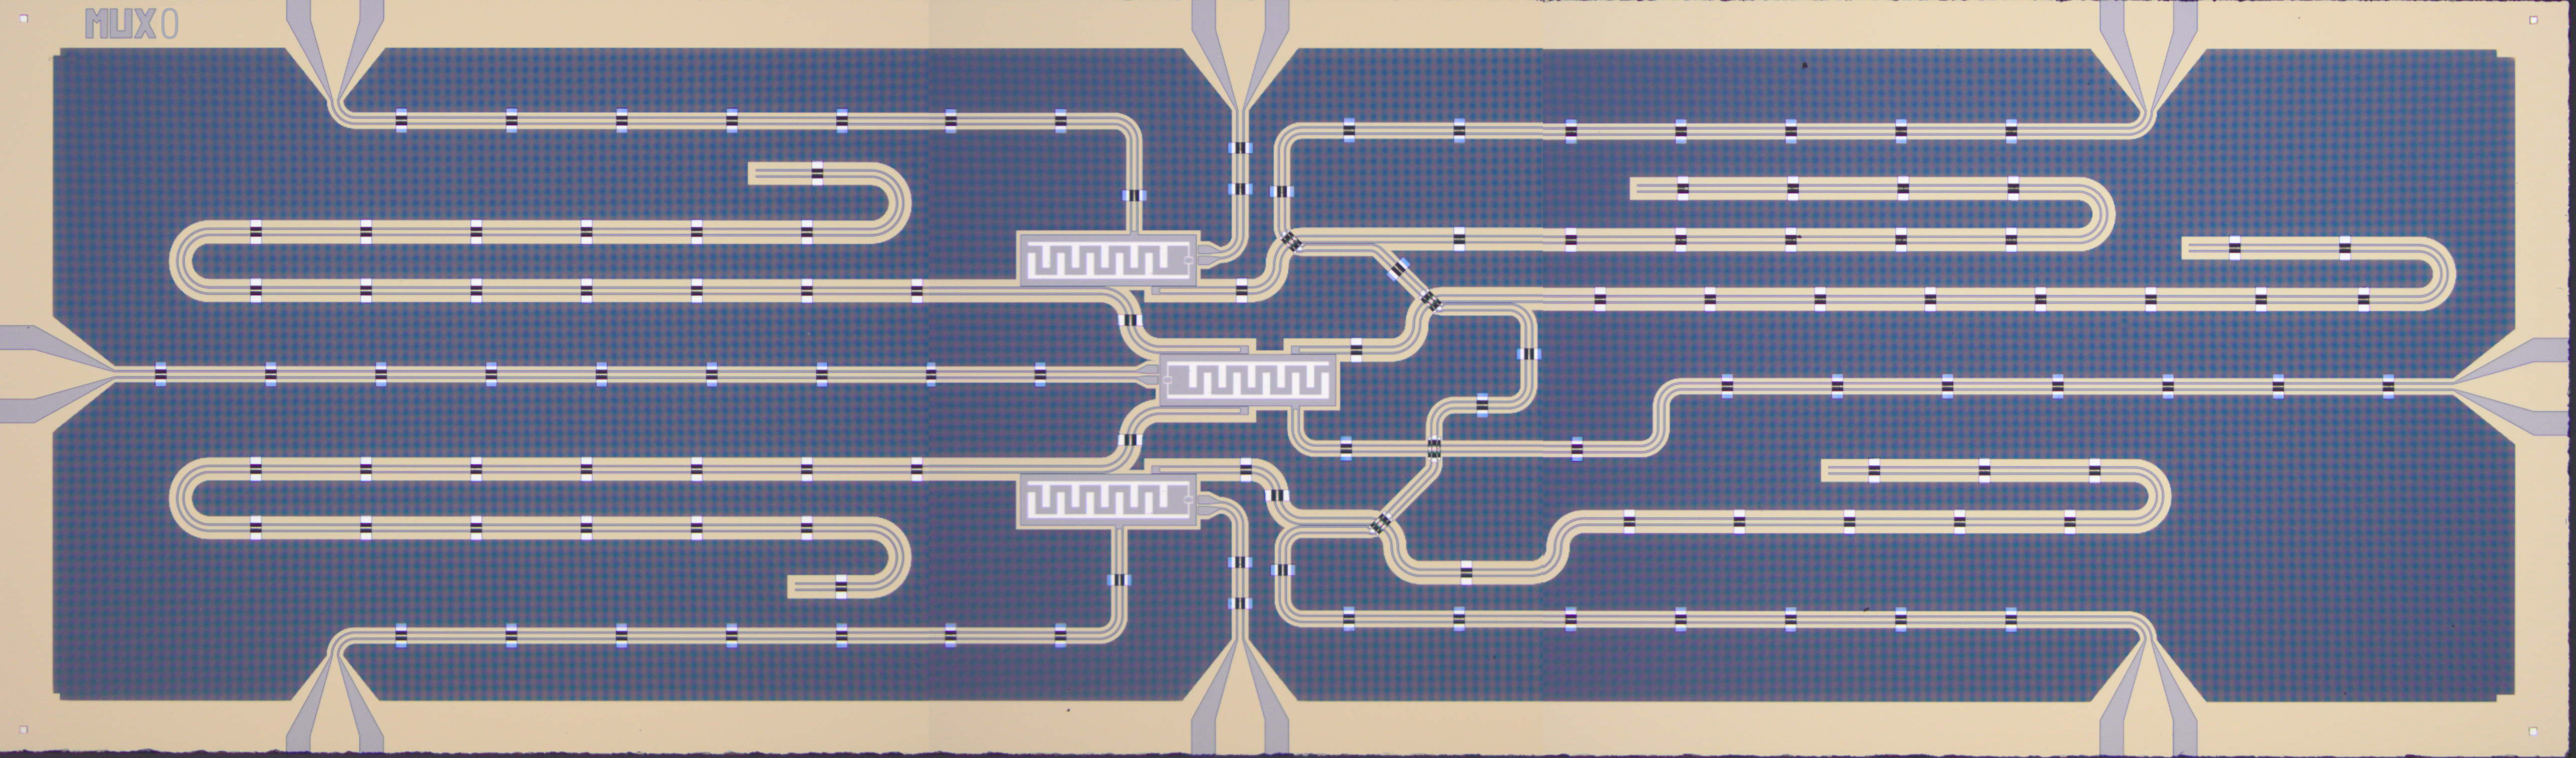
\includegraphics[width=1\linewidth]{../Figures/MUX_0.jpg}
          \caption{The Muxmon0 chip, in which the qubit drive lines are directly coupled}
          \label{fig:Muxmon0 image}
        \end{subfigure}

        \begin{subfigure}[b]{0.9\textwidth}
          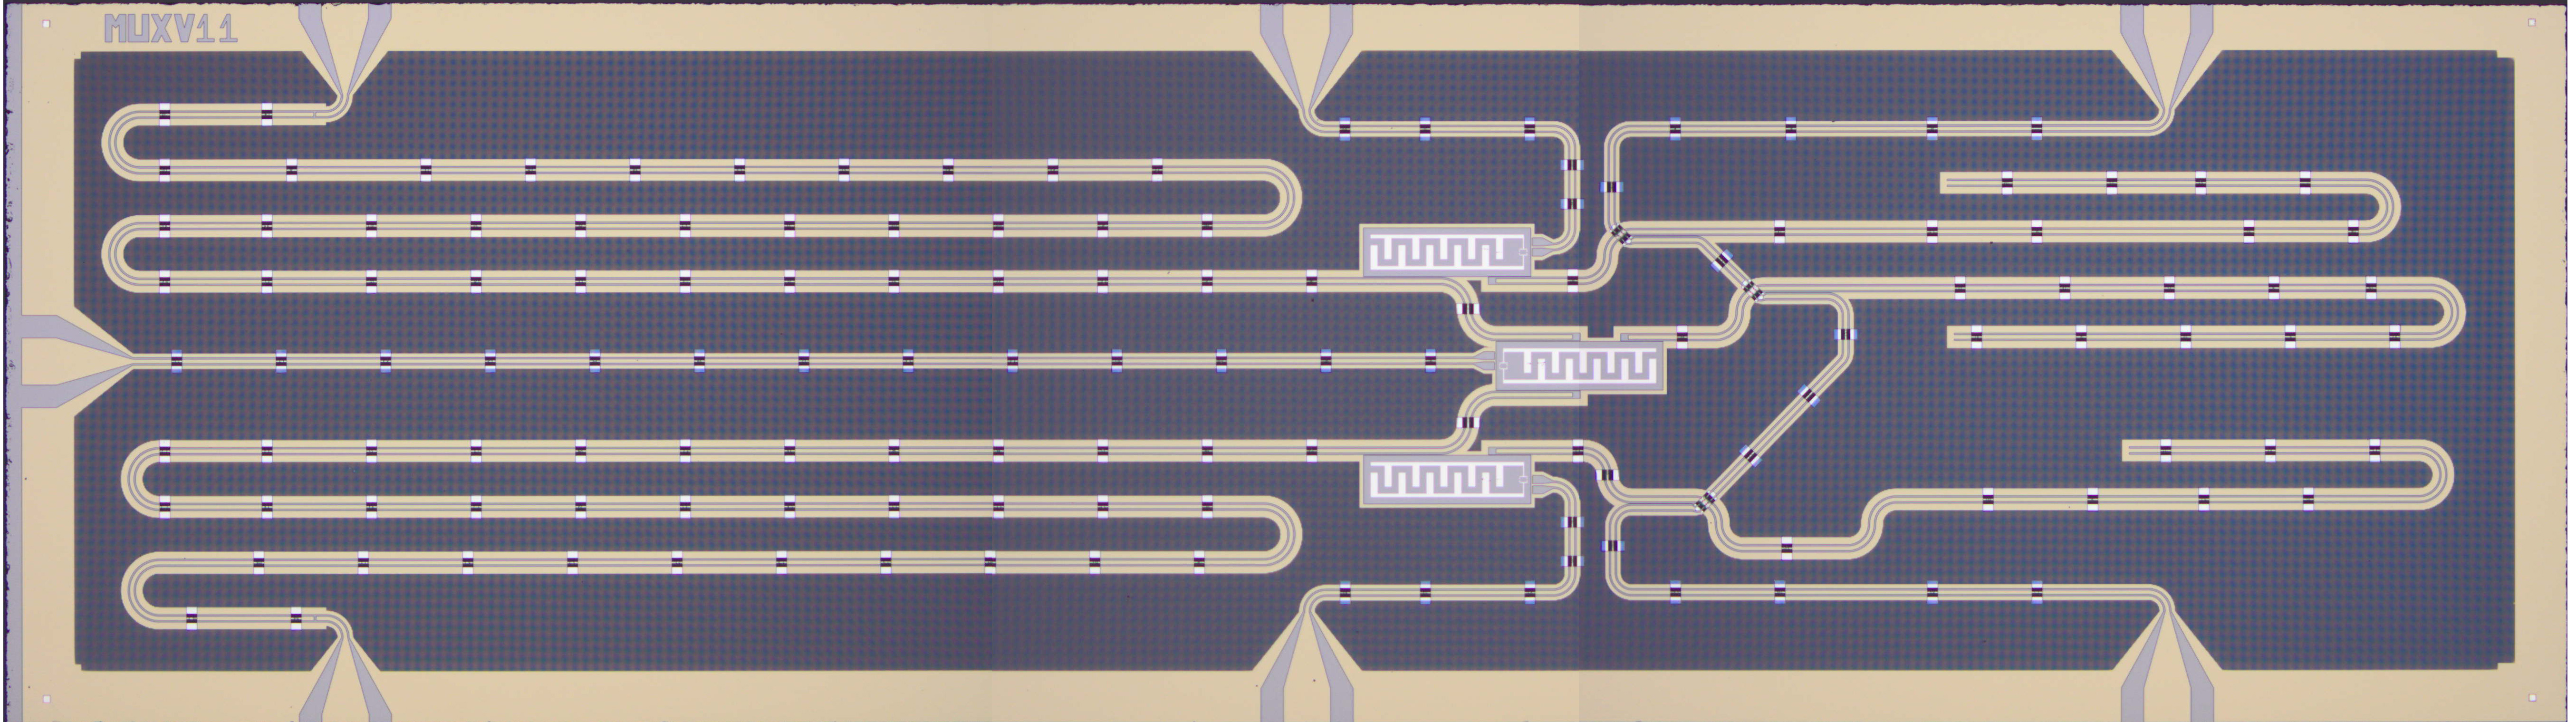
\includegraphics[width=1\linewidth]{../Figures/MUX_1.jpg}
          \caption{The Muxmon1 chip, in which the qubit drive lines are capacitively coupled}
          \label{fig:Muxmon1 image}
        \end{subfigure}
        \caption[Muxmon chips]{The Muxmon0 and Muxmon1 chips. The qubits of Muxmon0 have direct drive lines, while the qubits of Muxmon1 have drive lines capacitively coupled to the resonator buses.}
        \label{fig:Muxmon0 and Muxmon1}
      \end{figure}

      The Muxmon experiment was performed specifically to study frequency re-use and selective broadcasting using the Duplexer. Two chips were designed, Muxmon0 and Muxmon1, shown in Figure~\ref{fig:Muxmon0 and Muxmon1}. Both chips have three transmon qubits connected to them, all three of which are flux-tunable. Air-bridges are used, not only to connect the ground-planes in the coplanar waveguides, but also such that the feed line can cross over other lines. The key difference between the two chips is the approach used to drive the qubits In Muxmon0 all three qubits have their individual directly coupled drive lines. The top and bottom qubit are connected to the ancilla qubit through a bus. In the Muxmon1 the bus and drive lines are combined into two drive lines, each of which is capacitively coupled to the ancilla qubit and one of the other two qubits. The disadvantage of the direct drive lines in Muxmon0 is that they are an added decoherence channel for the qubits. However, the three drive lines of Muxmon0 ensure that individual qubit control of all three qubits is possible, even when they share the same frequency. This is in contrast to Muxmon1, where the ancilla qubit frequency must differ from that of the other two qubits. In the frequency re-use structure of the surface code, as explained in section\ref{sec:Frequency re-use in the Surface Code}, this should not be a problem, as frequency re-use in not applied to neighbouring qubits. Having capacitively coupled drive lines would result in less lines being required, both on-chip and outside the chip. Furthermore there would be one decoherence channel less. Therefore the capacitive coupled drive lines of Muxmon1 seemed the more attractive of the two options.

      During initial characterization of the qubits on both chips it was found that the coherence times of the qubits in Muxmon1 were considerably worse than those in Muxmon0 (see Appendix~\ref{sec:Muxmon1 coherence times}. It is, however, unlikely that this is due to the capacitively coupled drive lines, since one would expect the absence of direct drive lines to result in one less decoherence channel. Instead it is likely that the lower coherence times are simply due to some error in the chip fabrication process. Due to the lower coherence times of the qubits in Muxmon1, the focus of the experiment was on Muxmon0.

      \begin{figure}[tb]
        \centering
        \includegraphics[width=\textwidth]{../Figures/Muxmon set-up.pdf}
        \caption{The Muxmon set-up}
        \label{fig:Muxmon set-up}
      \end{figure}

      The Muxmon experiment set-up is shown in Figure~\ref{fig:Muxmon set-up}. Two of the four input ports of the Duplexer are used. One input port receives the main pulse, the other receives the DRAG pulse (see Section~\ref{ssec:qubit control} for more info). The main pulse and DRAG pulse are combined in the Duplexer. The output ports are connected to the drive lines of the top and bottom qubit.

  \chapter{Qubit characterization}
    \begin{description}
     \item[Description] This chapter gives a step-by-step description of how to find a resonator and qubit, and subsequently how to tune the qubit's parameters.
     \end{description}

    In the design of cQED chips, the parameters of the qubits and resonators are always targeted which are ideal for the experiment.
    For coplanar waveguide resonators one can already obtain relatively good parameters for the required dimensions from simple formulae \textbf{TODO:} refer to formula.
    For superconducting transmon qubits, however, finding the right dimensions that correspond to the desired parameters is a much more complicated process.
    The qubit's frequency, for instance, depends on the qubit's coupling energy $\Ec$ and Josephson energy $\Ej$. The coupling energy $\Ec$ can be reasonably estimated from classical simulations. Finding the right dimensions for the Josephson junction that result in the desired Josephson energy $\Ej$, however, is difficult, and usually physically testing different junctions is necessary to determine an accurate conversion from the desired $\Ej$ to the Josephson junction dimensions.

    Nevertheless, the actual parameters of the resonators and qubits are almost never where one expects them to be. Once the sample is cooled in the dilution refrigerator, an inevitable game of hide-and-seek follows with the goal of finding the frequency of the resonators and qubits, and subsequently determining their properties. This chapter describes the measurements that were performed to characterize the MuxMon samples.

    \section{Continuous-wave measurements}

      Once a sample is properly cooled down it is ready to be measured. At this stage the sample is still an unknown terrain, where the experimenter only has a rough map, containing the sample's targeted parameters, and the specific properties of the resonators and qubits.

      The first step is to look for signs of life. These manifest themselves as resonance frequencies of the resonators and the qubits that are coupled to them. As we are not yet interested in the properties of the resonators and qubits which can only be obtained through measurements with accurately timed pulses, we send continuous tones through the feedline, and measure deviations in the transmission. These measurements are known as continuous-wave measurements

      \subsection{Scanning for resonators}
        \label{sec:resonator-scan}
        Since communication with the qubits is mediated through their coupling to resonators, the first step is to find these resonators. This is done using a transmission measurement, in combination with heterodyne detection, and has been explained in section \textbf{TODO:} Create section in Resonator chapter.

        There is one difference in measuring a resonator when there is a qubit coupled to it. When considering the qubit as a two-level system, the behaviour of the coupled resonator-qubit system is governed by the Jaynes-Cummings Hamiltonian \cite{Reed}:

        \begin{equation}
          \hat{H} = \hbar \wres\left(\hat{a}^\dagger \hat{a} + \frac{1}{2} \right) + \frac{\hbar \wqub}{2}\hat{\sigma}_z + \hbar g \left(\hat{a}^\dagger \sigma_{-} + \hat{a}\sigma_{+}\right)
          \label{eq:Jaynes-Cummings}
        \end{equation}

        where $\wres$ is the bare resonance frequency of the resonator, $\wqub$ is the resonance frequency of the qubit's ground to excited state transition, and the qubit's two states are in the spin-representation. This Hamiltonian consists of three terms. The first term corresponds to the energy level of the resonator, the second to the energy level of the transmon, and the third is a coupling term between the two with coupling strength $g$.

        The difference between the resonator's frequency $\wres$ and the qubit's frequency $\wqub$ is given by the detuning $\Delta = \wqub - \wres$. If the magnitude of the detuning is large compared to the coupling strength $g$, the system is in the dispersive regime. In this case the Hamiltonian can be approximated by the dispersive Jaynes-Cummings Hamiltonian:

        \begin{equation}
          \hat{H} = \frac{\hbar \wqub^{'}}{2} \hat{\sigma}_z +  \left(\hbar \wres^{'} + \hbar \chi \hat{\sigma}_z\right) \hat{a}^\dagger \hat{a}
          \label{eq:dispersive-Jaynes-Cummings}
        \end{equation}

        The coupling between the qubit and resonator causes both qubit's frequency and the resonator's frequency to shift: $\wqub^{'} = \wqub + \chi_{01}$, $\wres^{'}=\wres - \chi_{12}/2$.

        Aside from experiencing a frequency shift dependent on the amount of detuning, Equation~\ref{eq:dispersive-Jaynes-Cummings} shows that the resonator also experiences a shift depending on the state of the qubit. The resonator's frequency is decreased by an amount $2 \chi$ when the qubit is in the excited state. The parameter $\chi$ is the dispersive shift, and is given by:

        \begin{equation}
          \chi = \chi_{01} - \chi_{12}/2 \approx \frac{g^2}{\Delta}\frac{\Ec}{\hbar \Delta - \Ec}
          \label{eq:dispersive-shift}
        \end{equation}

        where $\chi_{ij} = \frac{g_{ij}^2}{\omega_{ij}-\omega_r}$ are the partial dispersive shifts.

        Due to this coupling between resonator and qubit, it is important to choose the right RF power. When the amount of photons in the resonator reaches a certain point, this coupling will result in the resonator experiencing nonlinear effects. The resonator will thereby lose its Lorentzian lineshape. Therefore the RF power should be kept sufficiently low to avoid these nonlinear effects, while still maintaining a good signal-to-noise ratio.



        \textbf{TODO:}
        \begin{itemize}
          \item In the strong coupling regime (Leads to hybridization of qubit and resonator states: quton and fobit
          \item Explain that the quality factor is low because the resonator is coupled strongly to the qubit (equation including coupling to qubit?)
          \item Doesn't $\chi$ diverge when $\Delta \rightarrow \Ec$?
          \item explain concept of anharmonicity, and that $\alpha \approx E_c$
          \item Maybe explain concept of number splitting in dispersive Jaynes-Cummings. Number splitting is the phenomenon that the qubit's frequency shifts by an amount $2 \chi$ for every photon in the resonator.\\
                Alternatively mention this in another section.
          \item Mention that $g_{12}=\sqrt{g}$, and that other coupling strengths are exponentially suppressed in the transmon
        \end{itemize}

        \textbf{Figures:}
        \begin{itemize}
          \item Figure of transmission showing all three Muxmon0 resonators
        \end{itemize}

      \subsection{Powersweeping the resonators}
        \label{ssec:powersweep}

        \begin{figure}[tb]
          \centering
          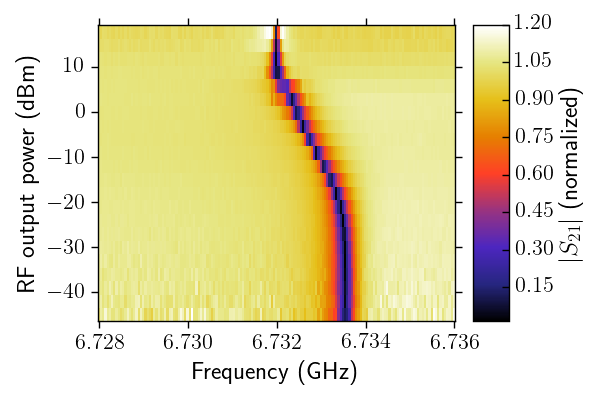
\includegraphics[width=0.6\textwidth]{../Figures/Qubit characterization/Powersweep.png}
          \caption{A powersweep of the resonator coupled to the ancilla qubit. The dispersive shift found is equal to $\chi\approx$\SI{30}{\mega \hertz}}
          \label{fig:powersweep}
        \end{figure}

        Once the resonators have been located, the next stage is to find the qubit that is capacitively coupled to each of the resonators. Instead of directly scanning the entire frequency spectrum in search of the qubit, it is relatively straightforward to perform some initial measurements aimed at gaining information about our resonator and qubit, which will allow us to search for our qubit with much greater accuracy.

        As explained previously, the capacitive coupling between the resonator and qubit shifts the resonator frequency $\wres$ from its bare frequency. When the amount of photons in the resonator reaches a certain point, the resonator experiences nonlinearity, thereby losing its Lorentzian lineshape. When increasing the RF power even further, at a certain point the resonator regains its Lorentzian lineshape. In doing so its resonance frequency has shifted to its bare frequency $\wbare$. If this frequency shift is observed, it indicates that the resonator's frequency was shifted, and hence that the qubit is alive. Measuring this frequency shift is commonly done in a powersweep. A powersweep is a measurement in which a resonator scan is performed for a range of powers.

        A powersweep additionally provides information about at what power the resonator enters the nonlinear regime. For measurements involving the qubit the readout power must be below this threshold power. Furthermore, from the frequency shift between the dressed cavity frequency and the bare cavity frequency, the amount of detuning between the qubit and the resonator can be estimated using Equation~\ref{eq:dispersive-shift}.

        If no shift is observed, it could mean that the qubit is dead (e.g. because the Josephson junction is shorted). However, this is not necessarily the case. An alternative possibility is that the detuning between qubit and resonator is very large, and as a result the frequency shift cannot be discerned. At this point it is too early to draw conclusions, and we may almost draw the analogy with Schr\"odinger's cat in a box.

        \textbf{TODO:}
        \begin{itemize}
          \item Explain theory behind transition to bare cavity frequency (Reed's thesis has some information)
        \end{itemize}

        \textbf{Figures:}
        \begin{itemize}
          \item Powersweep of ancilla qubit
        \end{itemize}

      \subsection{Scan for qubit sweet-spots}

        \begin{figure}[tb]
          \centering
          \includegraphics[width=.6\linewidth]{../Figures/Qubit characterization/Resonator vs DAC linecut.png}
          \caption{Fixed frequency transmission versus DAC current. The frequency is chosen to be slightly below the resonator frequency found when the DAC current is set to zero. The symmetry point in the linecut corresponds to the sweet-spot of the ancilla qubit.}
          \label{fig:figure1}
        \end{figure}
        Some of the qubits have a tunable resonance frequency. This is done through a superconducting quantum interference device (SQUID). In this case the two islands that compose the transmon qubit are connected by two Josephson junctions instead of one, effectively forming a loop. The SQUID loop is sensitive to the amount of flux passing through the loop. The amount of flux going through the SQUID loop can be changed by changing the surrounding magnetic field. This is commonly done by having a flux bias line in close proximity to the SQUID loop. Current flowing through the flux-bias line alters the magnetic field in the vicinity of the SQUID loop, and hence changes the amount of flux through the SQUID loop. A digital-to-analog converter is used to specify the amount of current that is sent through the flux bias line. Depending on the amount of flux through the SQUID loop, the resonance frequency of the qubit changes accordingly. these qubits are therefore called flux-tunable.

        For qubits that are flux-tunable, finding the sweet-spot of the qubit can be done without knowledge of the qubit's frequency. This can be done by sweeping the DAC voltage and measuring the shift in the resonance frequency. Because the frequency of the qubit varies as the amount of current through the flux-bias line changes, the detuning between the qubit and the resonator consequently changes. As a result the dispersive shift $\chi$, and therefore the resonator's frequency, also varies. At the sweet-spot of the qubit, the resonator's frequency $\wres$ is at a maximum. This is irrespective of whether the qubit's frequency $\wqub$ is above or below the resonator's frequency.

        The accurate way to measure the sweet-spot is to perform resonator scans as the DAC voltage is varied. The result is a 2D scan shown in \textbf{TODO:} Figure.

        A faster second approach for finding the qubit sweet-spot, at the cost of providing less information, is by choosing a fixed frequency close to the resonator's frequency $\wres$ (preferrably slightly below, where the transmission slope is steepest). By measuring the amount of transmission as the DAC voltage is being varied, one obtains essentially a line-cut of \textbf{TODO:} Figure. The idea this measurement is that if the qubit's frequency $\fqub$ decreases, the resonator's frequency also decreases, resulting in a decrease in transmission (closer to $\wres$). Likewise, if the qubit's frequency $\wqub$ increases, the resonator's frequency increases \textbf{TODO:} Why?, resulting in an increase in transmission (further away from $\wres$).

        At the qubit's sweet-spot, the resonator's frequency $\wres$ is at a maximum, and so the transmission should also be at a maximum. Furthermore, because the amount of detuning only depends on the deviation from the flux sweet-spot \textbf{TODO:} improve, the transmission should be symmetric with respect to the DAC voltage sweet-spot. If the resonator's frequency $\wres$ shifts by a large amount in the course of this measurement, it becomes harder to determine where the sweet-spot is (although even then often it can still be discerned). Nevertheless, this method is considerably faster than performing a full two-dimensional scan of frequency versus DAC voltage, and in most cases it works like a charm.

        In the case where the powersweep showed no measurable frequency shift, these two measurements are also useful in discerning whether or not the qubit is actually dead, or whether it was simply far detuned from the resonator.


        \textbf{TODO:}
        \begin{itemize}
          \item Explain how qubit's frequency has a cosine dependence on DAC
          \item Give detailed information on SQUID loop
          \begin{itemize}
            \item Why does the qubit frequency change in a SQUID loop
            \item Sweet-spot
          \end{itemize}
          \item Mention flux-noise?
          \begin{itemize}
            \item 1/f noise
            \item usually not limiting, as it is very slow
            \item This noise can be seen as occasional jumps (every few hours?) It would mean that every few hours the frequency must be recalibrated.
          \end{itemize}
        \end{itemize}

        \textbf{Figures:}
        \begin{itemize}
          \item SEM picture of SQUID loop, including flux-bias line
          \item Figure of 2D resonator scan vs DAC voltage
          \item Figure of 1D resonator fixed frequency DAC voltage scan
        \end{itemize}

      \subsection{Scanning for qubits}
        \label{sec:spectroscopy}
        Once the preliminary measurements have been performed that characterize the resonators and provide hints about the whereabouts of the qubit it is time to actually find the qubit.

        The measurement to perform in order to find the qubit depends on the amount of detuning between the resonator and qubit, which can be estimated from powersweep measurements. If the amount of detuning is large compared to the coupling strength ($\Delta \gg  g$), the system is in the dispersive regime. In this case one commonly performs a two-tone spectroscopy to find the qubit's frequency. If, on the other hand, the detuning is comparable to the coupling strength ($\Delta \sim g$), the qubit and resonator are hybridized, and experience an avoided crossing. In such cases a normal transmission measurement suffices.

        If the qubit is flux-tunable, one important question to ask is: at what DAC voltage should the qubit be searched?

        One option is to choose zero DAC voltage. In most cases this is alright, but there are cases when this is a bad choice. For instance, trapped magnetic fields during cool-down could position the qubit near the anti-sweet-spot for zero DAC voltage, in which case finding the qubit will be next to impossible.

        A better option is to choose a DAC voltage that results in a detuning $\Delta$ that is large compared to coupling strength $g$, such that the system is in the disperisive regime. However, the detuning $\Delta$ should not be too high, as it would otherwise result in a negligible dispersive shift $\chi$.The optimum value is usually around a few hundred megahertz, although this is dependent on the device-specific parameters. The detuning can be approximated using powersweeps.

        \subsubsection{Spectroscopy}
          As was explained in section~\ref{sec:resonator-scan}, in the dispersive regime the resonator experiences a $2 \chi$ frequency shift dependent on the state of the qubit. In the case of a resonator capacitively coupled to the feedline, the transmission experiences a dip at the resonator's frequency. This dip will correspondingly shift when the qubit's state is switched. The transmission at the resonator's dip when the qubit is in the ground state will therefore be dependent on the state of the qubit (low when the qubit is in the ground state, high when the qubit is in the excited state). This is the property exploited in a two-tone spectroscopy measurement.

          In a two-tone spectroscopy measurement two tones are sent through the feedline.
          \begin{enumerate}
            \item A drive tone with varying frequency $\wdrive$.
            \item A measurement tone at the resonator's frequency when the qubit is in the ground state.
          \end{enumerate}

          The transmission through the feedline is measured while the frequency of the drive tone $\wdrive$ is swept. When the drive frequency $\wdrive$ is detuned from the qubit's frequency $\wqub$, the drive is off-resonant with respect to the qubit, and so we measure a low transmission due to a dip being present. However, when the drive frequency $\wdrive$ approaches the qubit's frequency $\wqub$, then the qubit will start to oscillate between its ground and excited state, with a rate dependent on the detuning between the drive frequency $\wdrive$ and the qubit's frequency $\wqub$. The qubit will therefore have a partial population in the excited state, resulting in a shift of the resonator frequency, dependent on the population in the excited state. This is measured as an increase in transmission.

          The minimum linewidth of the qubit using spectroscopy is set by its dephasing time $T^2$, which can be seen as the uncertainty in its frequency. However, the power of the drive tone causes an additional increase in the linewidth, due to stimulated emission of the qubit. This effect is known as power broadening. This effect can be quite useful for finding qubits, especially when designing high-quality qubits with a very narrow intrinsic linewidth. The optimal power for the drive strength is further dependent on the amount of detuning $\Delta$ between the qubit and resonator. The resonator effectively acts as a bandpass filter, centered around the resonator frequency. Therefore, the stronger the detuning, the more the drive tone is suppressed.

          The dispersive shift $2 \chi$ is also dependent on the amount of detuning $\Delta$ between the qubit and resonator. If the detuning $\Delta$ is large, the dispersive shift will be very small, and so the difference in transmission will also decrease. Since the resonator has a Lorentzian lineshape, at the resonance frequency this Lorentzian is flat, and so is insensitive to small deviations. To increase the contrast between the on-resonant and off-resonant transmission, it is usually advantageous to measure at a slight detuning $\delta$ away from the resonance frequency, where the transmission slope is high. Since the resonator frequency shifts down when the qubit is excited, it is better to have a positive detuning $\delta$ to ensure that the transmission increases as the drive frequence $\wdrive$ approaches the qubit frequency $\wqub$ and decreases as it leaves the qubit frequency.

          \textbf{TODO:} Spectroscopy section
          \begin{itemize}
              \item Is power broadening really due to stimulated emission?
              \item Explain optimal RF power
              \item Is the gradual increase really due to partial population? Is it then an average of the partial population? Or do you get other effects as well?
          \end{itemize}


        \subsubsection{Avoided crossing}
          When the detuning $\Delta$ between the qubit and resonator is not large compared to their coupling strength $g$, the qubit and resonator experience an avoided crossing. Because all of the qubits in the Muxmon chips are considerably lower in frequency compared to their resonators, the system is always in the dispersive regime, and so the system never approaches the avoided crossing. Nevertheless it is worth mentioning the avoided crossing briefly, as it is a breeding ground for interesting physics.

          At the avoided crossing the system is not in the dispersive regime, and so the dispersive Jaynes-Cummings Hamiltonian no longer applies. In this case the resonator and qubit are hybridized, and one can no longer speak of a qubit and resonator as separate entities. Instead, this hybridization results in a so-called quton and phobit.

          \textbf{Avoided crossing info:}
          \begin{itemize}
            \item The coupling strength $g$ is the minimum distance be~tween the splitting
            \item From Reed's thesis p.63 explanation of this avoided crossing is given\\
            \begin{align}
             E_0 = & -\frac{\hbar \Delta}{2}\\
             E_1 = & n \hbar\omega_r \pm \frac{\hbar}{2}\sqrt{4g^2n + \Delta^2}
            \end{align}\\
            Joining $E_0 + E_1$ results in a qubit approaching a resonator from the top.\\
            When the frequency of the qubit equals that of the resonator, the energy difference reaches a minimum, and is equal to $2g$.
          \end{itemize}

          \textbf{TODO:} Avoided crossing
          \begin{itemize}
            \item Explain the quton fobit behaviour near the avoided crossing
            \item Explain how one can extract coupling from avoided crossing
            \item Explain that for the Muxmon qubit this effect is not present
            \item Explain multiple lines near avoided crossing
          \end{itemize}

          \textbf{figures:}
          \begin{itemize}
            \item Figure of avoided crossing
          \end{itemize}


        \textbf{TODO:}
        \begin{itemize}
          \item Use relatively high source power, results in power broadening
          \item Mention what to do if qubit is close to or far away from resonator
          \item Mention the term transmission measurement earlier on.
          \item Pulsed spectroscopy
        \end{itemize}

      \subsection{Tracking the qubits}
        \label{ssec:tracked spectroscopy}
        For flux-tunable qubits one is usually not interested in finding the frequency at one specific flux value. More important is finding how this frequency changes with varying flux. A naive approach would be to perform a two-dimensional scan of a fixed frequency range versus flux. At a certain flux the qubit crosses the boundary of the chosen frequency window. Every time this happens a new two-dimensional scan has to be performed with an updated frequency window. The larger the chosen frequency window, the less often this has to be updated. On the other hand, choosing a large window also means that a larger portion of the scan is spent not measuring the qubit. There is therefore a trade-off between measurement time and degree of human intervention. Furthermore, the resonator frequency also depends on the amount of detuning. Therefore the frequency of the measurement tone must also be updated every now and then.

        As an alternative approach I have created a modified version of the spectroscopy versus flux scan, known as tracked spectroscopy. In this approach after every spectroscopy scan the qubit frequency is extracted through fitting. From the qubit frequencies measured in previous scans the expected frequency at the next flux value is extrapolated. The frequency window of the next spectroscopy scan are then centered around the expected qubit frequency. The qubit is therefore tracked as its frequency changes. The same method is applied to update the resonator frequency.

        Tracked spectroscopy has several advantages over the two-dimensional spectroscopy versus flux scans. First of all, since the qubit's frequency follows a smooth curve (see Equation~\textbf{TODO:} Refer to eqn), the qubit's frequency can be estimated quite accurately. The frequency windows can therefore be narrow. This greatly reduces the measurement time. Secondly, tracked spectroscopy does not need any human intervention, as the frequency window is automatically updated after every spectroscopy scan. Therefore measuring the flux-dependence of the qubit frequencies is an automatized process (provided that the qubit frequency can correctly be extracted).

        For more information on the tracked spectroscopy algorithm see appendix~\ref{sec:Tracked spectroscopy}.

        \textbf{Improvements}
        \begin{itemize}
          \item Avoided crossing
          \item Variable RF and drive power
        \end{itemize}
        \textbf{TODO:}
        \begin{itemize}
          \item Maybe mention possible improvements
        \end{itemize}
        \textbf{Figures:}
        \begin{itemize}
          \item Tracked spectroscopy of qubit and resonator
        \end{itemize}

      \subsection{Finding the qubit's second transition}
        \label{ssec:12-transition spectroscopy}
        Once the qubit's grequency is known, it is possible to find the qubit's excited-state to second-excited-state transition $\omega_q^{12}$, which shall be referred to as the 12-transition. For consistent notation we shall temporarily denote the qubit's ground-state to excited-state transition frequency as $\omega_q^{01}$. The anharmonicity $\alpha$ is then given by the difference in transition frequencies: $\alpha = \omega_q^{12} - \omega_q^{01}$. Knowledge of the anharmonicity $\alpha$ allows determination of the coupling energy $E_c$ through \textbf{TODO:}.

        The 12-transition can be found using three-tone spectroscopy, in a manner similar to two-tone spectropscopy measurement explained in section~\ref{sec:spectroscopy}. The following three tones are used in three-tone-spectroscopy:

        \begin{enumerate}
          \item A drive tone with fixed frequency $\omega_\text{drive}^{01}$ at the qubit frequency $\omega_q^{01}$.
          \item A drive tone with varying frequency $\omega_\text{drive}^{12}$ to scan for the 12-transition.
          \item A third tone at the resonator frequency when the qubit is in the excited-state.
        \end{enumerate}

        The first drive tone with frequency $\omega_\text{drive}^{01}$ is used the drive the qubit to the excited-state. Since the first drive tone results in the excited-state being (partially) populated, the second tone with frequency $\omega_\text{drive}^{12}$ is then able to drive the qubit from the excited-state to the second-excited-state. The transmission should therefore change when $\omega_\text{drive}^{12}$ is on resonance with $\omega_q^{12}$.

        In principle the first drive tone with frequency $\omega_\text{drive}^{01}$ can be kept fixed at the 01-transition frequency $\omega_q^{01}$. However, by performing a two-dimensional scan, where $\omega_\text{drive}^{01}$ is also varied in a small region around $\omega_q^{01}$, the 12-transition becomes much clearer. This can be seen in \textbf{TODO:} Figure. Here a shift in transmission is observed when $\omega_\text{drive}^{01} = \omega_q^{01}$. This corresponds to the 12-transmission frequency $\omega_q^{12}$. Additionally, a transmission shift is observed at a line crossing $\omega_q^{12}$. At this line $\omega_q^{01} + \omega_q^{12} = \omega_q^{02}$, resulting in some population in the second-excited state.

        Once the 12-transition transition is found, and hence the qubit's anharmonicity $\alpha$, it is the possible to calculate the coupling energy $E_c$. \textbf{TODO:}.

        Finding the resonator frequency when the qubit is in the excited-state can be tricky, as pulsed spectroscopy is usually required. Nevertheless a rough estimation can be found using a modified version of spectroscopy, where the drive tone $\omega_\text{drive}$ is kept fixed, while the resonator frequency is swept. The lower peak will be a rough estimation of the resonator frequency when the qubit is in the excited-state. Alternatively it is also possible to use the resonator frequency when the qubit is in the ground-state, although this will reduce the contrast between driving on-resonance and driving off-resonance.

        It is worthwhile to note that three-tone spectroscopy produces much more accurate results when using pulsed spectroscopy, as the difference in transmission is generally small compared to two-tone spectroscopy.


        \begin{itemize}
           \item Coupling energy through solving Hamiltonian (see \cite{Reed}) .
        \end{itemize}

      \subsection{Flux matrix}
        \label{ssec:Flux matrix}
        When a current is passed through a flux-bias line, it is not only the flux through the SQUID of the qubit directly connected to it that is affected. Instead, the flux through SQUIDs of neighbouring qubits are also affected, albeit to a lesser extent. Therefore changing the frequency of one qubit by changing its corresponding flux-bias line current also affects the frequencies of the other flux-tunable qubits on the chip. For the Muxmon experiment the frequencies of the three qubits have to be individually tuned to very specific frequencies, and so the frequency responses of the qubits have to be decoupled. This is done by implementing a flux matrix, which corrects for the flux cross-coupling effects.

        A flux matrix $\boldsymbol{F}$ is an $n \times n$ matrix, where $n$ is the number of flux-tunable qubits. Each row corresponds to a virtual flux, and can be interpreted as follows: in a row $F_i = \left[f_{i1}, \dots, f_{in}\right]$ each element $F_{ij}$ corresponds to the relative amount by which the flux-bias line of qubit $j$ should be changed, such that only the frequency of qubit $i$ changes, while the frequencies of the other qubits remain fixed. This results in $n$ decoupled virtual flux parameters.

        Creating a flux matrix is done by first determining for each qubit separately how much every flux-bias line affects its frequency. For a given qubit $i$ this can be found by tuning the qubit away from its sweet-spot using its main flux-bias line, to a point where the slope $\partial f_i/\partial V_i$ of the qubit frequency $f_i$ as a function of DAC voltage $V_i$ is steep. This is the region where we are sensitive to changes in qubit frequency. For the main flux-bias line we already know from tracked spectroscopy what the slope $\partial f_i / \partial V_i$ is at this point. For each of the remaining flux-bias lines we measure the slope $\partial f_i / \partial V_j$ as we vary the DAC voltage $V_j$ and measure the response of the qubit frequency $f_i$. The slope $\partial f_i / \partial V_j$ is a measure for the amount of flux cross-coupling, which should be considerably less than for the main flux-bias line. Finally dividing all the slopes by the slope $\partial f_i / \partial V_j$ of our main flux-bias line, results in the ratio's of the frequency response of qubit $i$ for each of the flux-bias lines. Performing this measurement for all the qubits results in a matrix $\boldsymbol{M}$, where each element $M_{ij}=\partial f_i / \partial V_j$ is the normalized frequency response of qubit $i$ when varying the DAC voltage of the flux-bias line corresponding to qubit $j$. The diagonal elements of matrix $\boldsymbol{M}$ should be equal to one.

        Tracked spectroscopy provides accurate information on the DAC voltage corresponding to the sweet-spot of a qubit. The sweet-spot may not lie exactly at zero DAC voltage. It may shift due to magnetic flux being trapped during the cooldown of the fridge. These sweet-spots are usually found in the case where all the remaining flux-bias lines are set to zero DAC voltage. There is a certain combination of DAC voltages $\vec{V}^{ss}$ for which all the qubits are at their simultaneous sweet-spot. This simultaneous sweet-spot can be found using matrix $\boldsymbol{M}$. We know for each qubit $i$ the DAC voltage $V^0_i$ corresponding to its sweet-spot. Since $\boldsymbol{M}$ stores the amount by which each flux-bias line affects the flux of any qubit, the qubit $i$ remains at its sweet-spot as long as $\boldsymbol{M}_i \vec{V}=V^0_i$ holds, where $\vec{V}$ is the vector containing the DAC voltages. Therefore the simultaneous sweet-spot $\vec{V}^{ss}$ can be found by solving the set of equations $\boldsymbol{M} \vec{V}^{ss} = \vec{V^0}$, where $\vec{V}^0$ contains the DAC voltages of the individual sweet-spots of the qubits.

        The flux matrix $\boldsymbol{F}$ can be found by inverting matrix $\boldsymbol{M}$. As mentioned earlier, each row of matrix $\boldsymbol{F}$ corresponds to the ratio by which the DAC voltages of the flux-bias lines need to be varied, such that the frequency of only one qubit is changed. We may therefore multiply each row by a different constant, as long as the ratio between the elements in each row stays constant. One can normalizing each row such that the main flux-bias line is equal to one. This has the advantage that there is a one-to-one correspondence between DAC voltage and flux, and as a result the tracked spectroscopy will look identical. Additionally, after the normalization each row can be multiplied by a factor such that the virtual flux is equal to the flux quanta present in the SQUID loop. This conversion factor can be obtained by fitting the qubit frequency curve obtained from tracked spectroscopy.

        For a given virtual flux vector $\vec{\Phi}=\left[ \phi_1, \dots \phi_n \right]$, the corresponding DAC voltages $\vec{V}$ are given by:

        \begin{equation}
          \vec{V} = \boldsymbol{F} \vec{\Phi} + \vec{V}^{ss}
        \end{equation}

        By adding the simultaneous sweet-spot DAC voltages $\vec{V}^{ss}$, we obtain the additional property that the sweet-spot of the virtual fluxes is set to zero.

        After determining the flux matrix $\boldsymbol{F}$, there will still be some small remaining cross-coupling, which depends on the accuracy of the measurements. The process of creating a flux matrix can then be repeated, but instead of using DAC voltages as the varying parameters to construct matrix $\boldsymbol{M}$, the virtual fluxes should be used. Furthermore, as the cross-coupling is small compared to before, the flux range can be much greater, such that small slopes can be accurately measured. The resulting flux matrix $\boldsymbol{F}_2$ can then simply be multiplied with the first flux matrix $\boldsymbol{F}$ to obtain a more accurate final flux matrix.

    \section{Time-domain measurements}
      \subsection{Qubit control}
        \label{ssec:qubit control}
        So far the measurements described have all dealt with continuous tones being applied and measuring the response in the transmission. These are crude measurements, that are nevertheless able to determine some properties of the qubit and resonator, such as their frequencies. However, to find more detailed properties of the qubits, such as their coherence times, one cannot apply a continuous tone, that drives some incoherent qubit population. Instead well-calibrated pulses are required, which modify the state of the qubit in a precise manner, corresponding to gates being applied to the qubit. These types of measurements are called time-domain measurements, as they require precise pulse timing.

        A simple time-domain measurement usually consists of two parts. The first part consists of controlling the qubit. Here pulses are sent which modify the state of the qubit. The second part consists of measuring the state of the qubit. This is done through a readout tone, similar to spectroscopy measurements. This readout tone projects the state of the qubit onto the Z-axis. From the response in the transmission the state of the qubit can be inferred. More complicated experiments may involve some sort of feedback loop, where additional qubit control can be applied depending on the measurement outcome. These measurements require the qubit readout to be quantum non-demolition, i.e. the state of the qubit is not destroyed in the process of qubit readout. This usually involves extremely low-noise amplification, such as through a Josephson parametric amplifier. Feedback measurements are not performed in this experiment, and are therefore beyond the scope of this thesis.

        Qubit pulses usually have a Gaussian shape. These pulses can be generated by modulating a carrier signal from an RF generator, and is commonly done using an Arbitrary Waveform Generator (AWG). For the Muxmon experiment the Tektronix AWG5014 is used, which has four channels, each of which can control its voltage output at the nanosecond scale. It further has eight marker channels, which can be used to trigger devices, such as RF generators and the Duplexer. The carrier signal is sent through the LO port of the mixer, and an AWG channel is connected to the IF port of the mixer. The ouput at the RF port of the mixer is the modulated signal, the amplitude of which depends on the amplitude of the AWG channel output.

        For IQ mixers it is also possible to modulate both quadratures of the carrier signal independently, using two AWG channels. This allows for single sideband modulation, which is done by convoluting the pulses of the I and Q quadrature channels with a sine and cosine respectively. The sideband modulation frequency $\omega_{sb}$ of these sinusoidal functions is the amount by which the carrier signal is shifted. Single sideband modulation has the advantage that the carrier frequency $\omega_c$ is shifted away from mixer leakage, which would otherwise cause a slight continuous rotation of the qubit. For more information on mixer leakage, see section~\ref{sec:Mixer calibration}.

        The length of the pulse is an important consideration. Shorter pulses allow for more qubit operations within its coherence time. On the other hand, the shorter a pulse is in time, the larger its frequency spectrum will be. At a certain point the spectrum will be so broad that there will be a nonnegligible signal at the qubit's excited-state to second excited-state transtion frequency. This will cause leakage to the second excited-state, thereby leaving the two-state Hilbert space.
        Furthermore, the finite resolution of the AWG causes the pulses to be discretized, resulting in the pulses being slightly distorted. The shorter the length of the pulse, the more discretization, and therefore distortion, will occur. This can cause further leakage to the second excited-state. It is therefore desirable to have a bandwidth, which is the inverse of the width $\sigma$ of the Gaussian pulse, that is small compared to the anharmonicity of the qubit.

        A second pulse, known as the Derivative Removal by Adiabatic Gate (DRAG) pulse \cite{motzoi2009simple}, can be applied along with the main pulse, to reduce the amount of leakage. The DRAG pulse is the derivative of the main Gaussian pulse, and adiabaticaly populates the second excited state during the pulse, and subsequently withdraws this population back to the two-state Hilbert space. Using the DRAG pulse can reduce the amount of leakage by orders of magnitude.

        \textbf{TODO:}
        \begin{itemize}
          \item Explain about the measurement process, and that many averages need to be performed to get an accurate estimate of the qubit state $\sqrt{N}$. This is important for single-shot measurements later on
          \item Explain more on Z projection
          \item Explain more on non-demolition.
          \item Signal quadrature determines the rotation angle
          \item Mention that AWG channel amplitude must not be too high, and that attenuation should be used to avoid spurious resonant modes
          \item Refer to Noise chapter for more information on single sideband modulation?
          \item Mention that amount of rotation depends on time duration, refer to Reed's thesis
        \end{itemize}

        \textbf{Questions:}
        \begin{itemize}
          \item Are both quadratures modulated independently in IQ mixers?
          \item Why use sideband modulation?
          \item Why are Gaussian pulses used?
         \end{itemize}

         \textbf{Figures:}
         \begin{itemize}
            \item Gaussian pulse with derivative
          \end{itemize}

      \subsection{Drive amplitude calibration}
        \label{ssec:Rabi}
        Performing gates on qubits requires knowledge of the parameters that define the pulse, such as the amplitude, phase, and pulse duration. The phase determines the axis along which the qubit is rotated. The duration and amplitude of the pulse determine the rotation angle. To rotate the qubit by a specific angle, either the pulse duration can be varied, keeping the amplitude fixed, or the pulse amplitude can be varied, keeping the pulse duration fixed. Both methods have advantages and disadvantages. Varying the pulse duration ensures that the maximum amplitude is roughly fixed, regardless of the rotation angle. On the other hand, pulses with a small rotation angle have a very small duration, and so their bandwidth will be large, which may lead to increased leakage. Varying the amplitude, on the other hand, ensures that pulses applied to multiple qubits end simultaneously, and so it is more natural to speak of a pulse clock cycle. In the measurements for this thesis the amplitude is varied, while the pulse duration is kept fixed.

        Determining the correct amplitude for qubit gates is commonly performed using a Rabi measurement. In this measurement the amplitude of a pulse with rotation along the X-axis is varied monotonically. The pulse will cause the qubit to rotate at a Rabi rate $\Omega_R$, which depends on the pulse amplitude.

        After application of a pulse with Rabi rate $\Omega_R$ and duration $\tau$, the wavefunction will be in state $\ket{\psi} = \cos{\left( \frac{\Omega_R}{2} \tau \right) } \ket{0} + \sin{\left( \frac{\Omega_R}{2} \tau \right)} \ket{1}$. After a measurement the qubit will be in the excited state with probability $\sin^2{\left( \frac{\Omega_R}{2} \tau \right)}$ \cite{Reed}. The Rabi rate $\Omega_R$ is proportional to the pulse amplitude.

        In a Rabi measurement the amplitude is swept monotonically from a negative value to a positive value. The result should look like a cosine, as shown in Figure \textbf{TODO}. The center of this cosine is where the amplitude is zero, and therefore corresponds to the ground-state of the qubit. At the other peaks, where the deviation from the ground-state is the largest, the qubit is in the excited-state. The amplitude of the left peak corresponds to a negative pi-pulse, and the right peak to a positive pi-pulse. Usually the amplitude step between successive segments is tuned such that the excited-state peaks are at specific segments.

        \textbf{Questions:}
        \begin{itemize}
          \item How does the rotation angle depend on the amplitude?
        \end{itemize}
        \textbf{TODO:}
        \begin{itemize}
          \item time variation or amplitude variation
          \item Refer to equation showing that rotation depends on time duration (Reed's thesis)
        \end{itemize}

      \subsection{Qubit decoherence}

        \subsubsection{Qubit relaxation: T1}
          Once a pi-pulse has been tuned it is possible to excite the qubit. However, once the qubit is excited, it will not remain so indefinitely. Instead, the excitation will slowly leak away to different relaxation sources, some of which have been discussed in \ref{sec:Losses}. These sources of relaxation lead to an exponential decay of the qubit's excitation, with a relaxation time $T_1$. This relaxation can be visualized on the Bloch sphere as the stateA typical measurement to characterize the relaxation time $T_1$ is performed by first applying a pi-pulse, and the waiting for a monotonically increasing wait time $\tau$, after which the state of the qubit is measured.

          relaxation time $T_1$,

          \begin{itemize}
            \item Purcell limit
          \end{itemize}


        \subsubsection{Qubit dephasing: Ramsey}
          \label{sssec:Ramsey}
          Aside from relaxation, the qubit also experiences another form of decoherence, namely dephasing, resulting from phase noise. Phase noise can be seen as fluctuations in the qubit frequency. It is characterized by the dephasing time $T_2^*$. The dephasing time $T_2^*$ has an upper bound equal to $2\;T_1$ \cite[pp56-58]{Bishop}, but can decrease significantly due to other sources of phase noise, such as charge noise, fluctuating cavity photon number, and flux noise for flux-tunable qubits \cite[p126]{Sears}. Qubit dephasing results in a random phase being added to the qubit, and can be visualized on the Bloch sphere as the transversal component of the qubit's state decreasing in magnitude, as the qubit's phase has increased uncertainty. In the limiting case this will result in all phase information being lost, with the qubit's state thereby lying on the Z-axis.

          One method of measuring the dephasing time $T_2^*$ is by performing a Ramsey measurement. A Ramsey sequence consists of an initial $X_{\pi/2}$ pulse, after which the qubit lies on the equator of the Bloch sphere. After a certain wait time $\tau$, a second $X_{\pi/2}$ pulse is applied to the qubit. The combination of the two pulses should result in the qubit ending up at the excited-state. However, during the wait time $\tau$ the qubit experiences dephasing, causing it to deviate from its original position on the equator. Therefore the final state of the qubit will deviate from the qubit's excited-state. The probability of the final state to end up in the excited-state has an exponential decay, asymptotically approaching $0.5$ (all phase information lost).

          During the wait time $\tau$, when the qubit lies on the equator, it does not only experience dephasing. When the frequency of the driving tone $\omega_d$ is different from the qubit frequency $\omega_q$, the qubit will precess along the equator with a frequency equal to the Rabi rate $\Omega_R = \omega_d - \omega_q$. At the moment we ignore effects such as decoherence and gate errors. The first pulse results in the qubit being at the equator. If there were no precession, the result of the second pulse is that the qubit is in its excited-state. However, any detuning $\Delta$ causes the state of the qubit to deviate from the excited-state. In fact, after half a period the second pulse results in the qubit being in its ground-state. After one full period, however, the qubit has returned to its original position on the equator, and so the second pulse will result yet again in the qubit being in its excited-state.

          In a Ramsey measurement the final state of the qubit is measured as the wait time $\tau$ between the two pulses is monotonically increased. The result should exhibit an oscillatory behaviour, the frequency of which being equal to the Rabi rate $\Omega_R$. Furthermore, dephasing causes this oscillation to decay exponentially, at a rate $1/T_2^*$. The excited-state population $P_1$ as a function of wait time is given by:

          \begin{equation}
            P_1(t) = e^{t/T_2^*} * \cos{\left( 2 \, \pi \, \Omega_R \, t \right) + 1/2}
            \label{eq:Ramsey}
          \end{equation}

          Usually in a Ramsey measurement artificial detunining is added to the pulse, such that if there were no real detuning, one would see around three to four oscillations. There are several reasons for this artificial detuning. One reason is that estimating the detuning using Equation~\ref{eq:Ramsey} is more accurate once there are several oscillations present. Another reason is that if the real detuning is reasonably small compared to the artificial detuning, it is possible to estimate if the qubit's frequency is higher or lower than the drive, as this would result in a higher or lower oscillation frequency.



          \textbf{Questions:}
          \begin{itemize}
            \item Where does exponential noise and Gaussian noise come from? As I understand it Gaussian noise is due to flux
            \item Is $T_1$ not noticeable in a Ramsey measurement?
            \item Why is maximally $T_2^*=2T_1$?
          \end{itemize}

          \textbf{Figures:}
          \begin{itemize}
            \item Ramsey measurement
            \item $T_2^*$ vs. frequency?
          \end{itemize}

        \subsubsection{Fast frequency qubit dephasing: Echo}
          The dephasing time $T_2^*$ is a combination of several different phase noise sources. Some of these sources produces high frequency (fast) noise, while others produce low frequency (slow) noise. It is possible to distinguish these two effects by performing a second dephasing measurements that filters out slow noise, called an Echo measurement.

          An Echo measurement is quite similar to a Ramsey measurements, where two $X_{\pi/2}$ pulses are applied, separated by a wait time $\tau$. The difference is that in the middle of this wait time, at $\tau/2$, an additional refocusing $X_{\pi}$ pulse is sent. This has the effect that the state of the qubit is essentially flipped on the Bloch sphere around the X-axis. Any slow phase noise, which we can view to be quasi-static, is thereby cancelled. Fast phase noise, however, will vary considerably during the wait time $\tau$, and so will still cause dephasing. In the absence of decoherence, the final state of the qubit is the ground-state, which is in contrast to a Ramsey measurement, where the final state is the excited-state.

          An Echo measurement is performed by monotonically increasing the wait-time $\tau$, while keeping the three pulses relative to the wait time $\tau$ fixed. The result is similar to a Ramsey measurement, showing an exponential decay, with corresponding Echo dephasing time $T_2^E$. This value should be higher or equal to the dephasing time $T_2^*$. The refocusing pulse has the additional effect that any precession due to detuning is also cancelled. This inhibits the oscillatory behaviour that is present in Ramsey measurements. To be able to better estimate the Echo dephasing time $T_2^E$, the phase of the final $X_{\pi/2}$ pulse is monotonically shifted, such that the result is an oscillation in qubit state.

          There are more complicated Echo sequences, involving multiple refocusing pulses. By placing these at specific times the different frequency contributions of the phase noise can be characterized. Furthermore, by repeatedly applying a refocusing pulse, the state of the qubit can be preserved much longer than the limit imposed by $T_2^*$.


          \begin{itemize}
            \item $T_2^E$ Should be larger than $T_2^*$
          \end{itemize}

          \textbf{Figures:}
          \begin{itemize}
            \item Echo measurement.
          \end{itemize}

      \subsection{Measuring single shots}

  \chapter{Calibration routines}
    \textbf{TODO:} Introduction
    \section{Accurate frequency estimation}
      Spectroscopy provides an estimate for the frequency of the qubit. However, even with pulsed spectroscopy, the accuracy is limited to roughly a megahertz. When the frequency of the driving tone $\omega_d$ is different from the qubit frequency $\omega_q$, the qubit will precess around the Z-axis with a frequency equal to the Rabi rate $\Omega_R = \omega_d - \omega_q$. As explained in Section~\ref{sssec:Ramsey}, this detuning is measured in a Ramsey measurement, where the qubit frequency can be inferred from the precession rate.

      A Ramsey measurement provides a very accurate estimate for the qubit frequency $\omega_q$. The longer the wait time $\tau$, the more the qubit precesses around the equator. Therefore tiny differences between the drive frequency $\omega_\text{drive}$ and the qubit frequency $\omega_q$ can be detected. The upper bound on the accuracy of being able to determine the qubit frequency is set by the qubit's dephasing time $T_2^*$. This is because the dephasing time $T_2^*$ corresponds to the fluctuation in the qubit frequency.

      The main goal of the Muxmon experiment is to measure the performance of space-division multiplexing using the Duplexer. One requirement for space-division multiplexing is that the top and bottom qubit are at the same frequency. Any effect due to weak coupling between the qubits is only present if the two qubits are accurately tuned to the same frequency. Furthermore, since only a single frequency will be used, any detuning will lead to a decrease in qubit performance. To this end the top qubit has been detuned from its sweet-spot, to match the bottom qubit, while both the bottom and ancilla qubit are kept at their respective sweet-spots. This process is greatly simplified through use of a flux matrix, as described in section~\ref{ssec:Flux matrix}. Initial top qubit frequency tuning was done using spectroscopy, which is a much faster measurement. After the initial frequency tuning, accurate frequency tuning was performed using Ramsey measurements. First the bottom qubit frequency $\omega_q^B$ was determined, after which the top qubit frequency $\omega_q^T$  was tuned to match $\omega_q^B$. This process has been fully automatized. Using this method the inidividual frequencies could be determined to within \SI{10}{\kilo \hertz}, and the two frequencies could be tuned to within \SI{50}{\kilo \hertz} of one another. The reason the frequencies could not be tuned more accurately is due to the IVVI having a finite DAC voltage stepsize.

      \textbf{Questions:}
      \begin{itemize}
        \item What is the resolution of the IVVI? To what qubit frequency difference does this correspond for the top qubit?
      \end{itemize}

    \section{Accurate drive amplitude calibration}
      \label{sec:PiX360}
      To test the limits of performance using the Duplexer all gates need to be calibrated to a very high accuracy. The Rabi measurement explained in section~\ref{ssec:Rabi} is able to tune the drive amplitude up to a certain degree. However, the degree to which one can tune the drive amplitude using Rabi is limited, and for fine-tuning different methods are required.

      In the Muxmon experiment, the method used for accurate drive amplitude calibration is based on applying repeated pi-pulses on the qubit. The entire sequence can be summarized as $\left( X_{\pi} \right)^{2N} X_{\pi/2} \ket{0}$, where $N$ is the segment number. In the absence of gate errors and decoherence, the qubit should return to the equator, regardless of the segment number $N$. However, any amount of overdriving or underdriving results in small rotations that are added coherently, resulting in a positive or negative slope respectively. These slopes serve as very accurate measures for the optimal drive amplitude. If the difference in driving strength is large, oscillations will be present, corresponding to rotations around the Bloch sphere.

      % The $X_{\pi/2}$ pulse at the start of the sequence provides two benefits. The first is that any slope is clearly visible, since the final state is projected onto the Z-axis. Secondly, relaxation effects are to a certain extent
      % \begin{itemize}
      %   \item Accurate drive amplitude calibration using PiX360
      %   \item PiX180 is also possible, but PiX360 has added benefit of having all points in a continuous line
      %   \item PiX360 furthermore achieves higher accuracy, as there are fewer pulses
      %   \item PiX180 however can be performed at larger detuning, due to slower oscillations
      %   \item Much better accuracy than Rabi
      %   \item Pi/2 pulse at start of sequence instead of at end
      %   \item If at end, T2 effects are less
      %   \item If at start, T1 effects are less
      %   \item Additional performance increase could be achieved by individually calibrating other pulses
      % \end{itemize}

      \textbf{Figures:}
      \begin{itemize}
        \item PiX360 with positive, normal, negative slope
      \end{itemize}

    \section{DRAG parameter calibration}
      The DRAG parameter has been calibrated by measuring the difference in signal between an $X_{\pi} Y_{\pi/2}$ pulse and a $Y_{\pi} X_{\pi/2}$ pulse. Ideally for both pulses the final state should lie on the equator. However, an incorrectly tuned DRAG parameter would result in the first pulse to rotate the qubit slightly toward the excited-state, while the second pulse would rotate the qubit slightly toward the ground state. The DRAG parameter is found by minimizing this difference.

      \textbf{Questions:}
      \begin{itemize}
        \item Why does this produce errors in opposite direction?
      \end{itemize}

    \section{IQ mixer calibration}
      \label{sec:Mixer calibration}

      \begin{figure}[tb]
        \centering
        \begin{subfigure}[h]{0.49\textwidth}
          \caption{}
          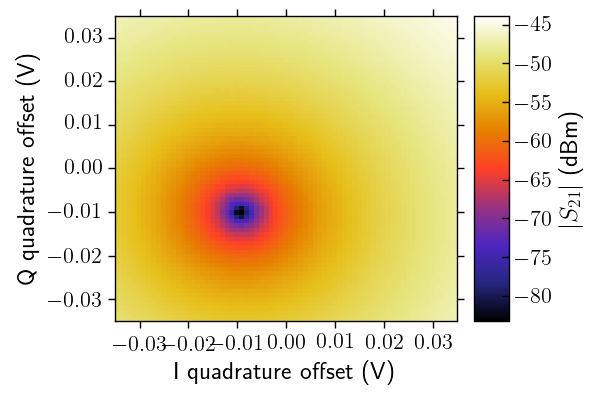
\includegraphics[width=\textwidth]{../Figures/Calibration routines/Mixer offset.png}
        \end{subfigure}
        \begin{subfigure}[h]{0.49\textwidth}
          \caption{}
          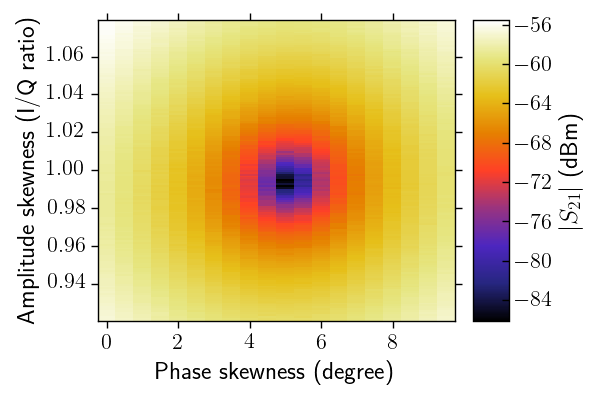
\includegraphics[width=\textwidth]{../Figures/Calibration routines/Mixer skewness.png}
        \end{subfigure}
        \caption{Mixer carrier leakage (a) and mixer skewness (b). Without any corrections both the mixer carrier leakage and the signal due to mixer skewness are equal to \SI{-58}{\dBm}. Compared to the main signal with output power equal to \SI{-32}{\dBm}, the mixer imperfections would result in two additional signals, each with strength \SI{-26}{\dB}.}
        \label{fig:Mixer calibrations 2D}
      \end{figure}

      An important calibration routine which must not be forgotten is correcting for mixer imperfections. there are mainly two \textbf{TODO:} that must be calibrated in an IQ mixer: the mixer carrier leakage, and the mixer skewness.

      For a perfectly balanced mixer, a signal of given frequency $\omega_0$ at the LO port should produce no output at the RF port if no modulation signal is applied in the inphase and quadrature ports.  However, any imperfections, due to for instance diode mismatches in the mixer, may lead to some signal at frequency $\omega_0$ leaking through. This leakage can be compensated to a large extent by adding a DC offset to the inphase and quadrature IF signals leaving the AWG, for which the leakage is minimized. Determining the optimal DC offset can be performed by sending a carrier signal into the LO port of the mixer, and a continuous DC signal from the AWG to both IF ports of the mixer. The leakage can be measured as signal exiting the RF port at the carrier frequency $\omega_0$, and can be minimized by varying the offsets of the individual AWG channels.

      Another type of IQ mixer imperfection is mixer skewness. The carrier signal entering the LO port is split into its inphase and quadrature component, where it is mixed with an inphase and quadrature IF signal. Ideally the inphase and quadrature components of the LO signal are perfectly orthogonal. However, in reality this is not the case, and so a small amount of skewness is present. Ideally the signal should be shifted in frequency to the desired sideband frequency $\omega_0 + \omega_{sb}$. However, any mixer skewness will lead to the signal being partially shifted in the opposite direction, resulting in some signal at the unwanted sideband frequency $\omega_0 - \omega_{sb}$. Additionally any amplitude skewness between the two IF ports will also result in signal at the unwanted sideband frequency. The signal at the unwanted sideband can be measured for a given carrier frequency $\omega_0$ by adding a sine and cosine with sideband frequency $\omega_{sb}$ to the inphase and quadrature ports respectively.   This can be corrected during the generation of the pulses through a transformation $\left( I, Q \right) \rightarrow \left( I', Q' \right) = \left( I - Q \tan{\phi}, Q \sec{\phi} \right)$, where $\phi$ is the phase skewness. The skewness can be corrected by varying the phase and amplitude of one of the AWG channels, and minimizing the signal at the unwanted sideband. The inphase and quadrature signals have to be transformed for every phase. Note that the mixer skewness is dependent on both the carrier frequency $\omega_0$ and the sideband modulation frequency $\omega_{sb}$

    \section{Duplexer phase calibration}
      \label{sec:Duplexer phase calibration}
      The Duplexer has phase-shifters for each of input-output combinations. That means that the phases of each of the eight channels can be tuned individually.. In the case of the Muxmon experiment, where we have independent control over the main pulse and the DRAG pulse, we require the two channels to share the same phase. The phase of two Duplexer channels can be tuned to one another by sending two signals with opposite phase into the Duplexer. If the relative phase shift of these two signals induced by the Duplexer, these two signals should (partially) cancel each other, resulting in a dip in transmission. The amount of transmission at this dip depends on the amplitude difference between the two signals.

      Calibrating the Duplexer phase can be done by splitting a signal from an RF generator, and then using single sideband modulation on both signals individually, where the phase of one of the sidebands is shifted by $180 \degree$, which can be realized using an AWG. As the phase of one of the channels is varied, a dip in transmission corresponds to both Duplexer channels sharing the same phase shift.

    \section{Readout calibration}
      \label{sec:Readout calibration}
      Should I include this?

    \section{AllXY}
      \label{sec:AllXY}
        There is a good measurement to test how well the qubit has been tuned, namely the AlllXY measurement. This measurement consists of all 21 possible two-gate combinations of $\left\{Id, X_{\pi}, Y_{\pi}, X_{\pi/2}, Y_{\pi/2}\right\}$. Each combination is susceptible to different types of gate errors to a different degree. The AllXY combinations have therefore been arranged in such a way that the final state of the first five combinations is the ground-state, the final state of the second twelve combinatios is the equator, and the final state of the last four combinations is the excited-state. Furthermore the combinations are arranged in such a way that the most common sources of gate errors can be distinguished. The full list of combinations in correct order can be found in App~\ref{ssec:AllXY}.

        The errors that can be distinguished are extensive: drive amplitude, DRAG parameter, frequency detuning, signal reflections, and several more. This is the strength of AllXY, but simultaneously its weakness. If there are multiple errors present, their errors may interfere, resulting in symptoms which are difficult to diagnose. nevertheless, it is a powerful tool, especially if one source of gate error is dominant. For a detailed analysis of the AllXY symptoms produced by different types of gate errors, see Reef~\cite{Reed}.

      The Duplexer can modify the signal of each of its input-output port combinations individually. In the set-up used for the Muxmon experiment, both the drive amplitude and DRAG parameter can be separately tuned for each of the two qubits. In Figure~\ref{fig:AllXY individual control} the AllXY results are shown for the top and bottom qubits, as the drive amplitude and DRAG parameter of the top qubit is varied using the Duplexer. As can be seen there is no noticeable change in the AllXY of the bottom qubit, even though the top qubit's performance changes considerably. This shows that the Duplexer allows for individual drive amplitude and DRAG parameter control for each qubit, without affecting the other.

      \begin{figure}
      \centering
         \begin{subfigure}[b]{\textwidth}
         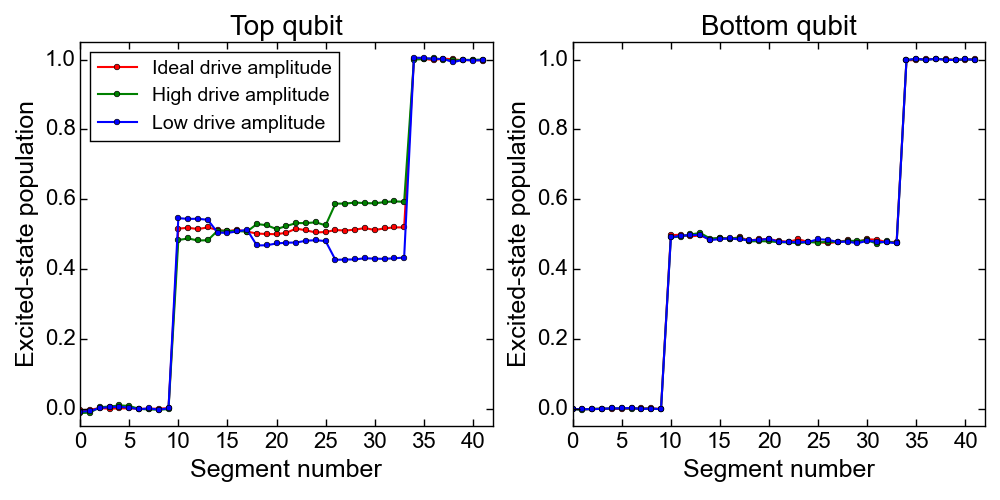
\includegraphics[width=1\linewidth]{../Figures/Exploring frequency re-use/AllXY_drive_top.png}
         \caption{}
         \label{fig:AllXY drive top}
      \end{subfigure}

      \begin{subfigure}[b]{\textwidth}
         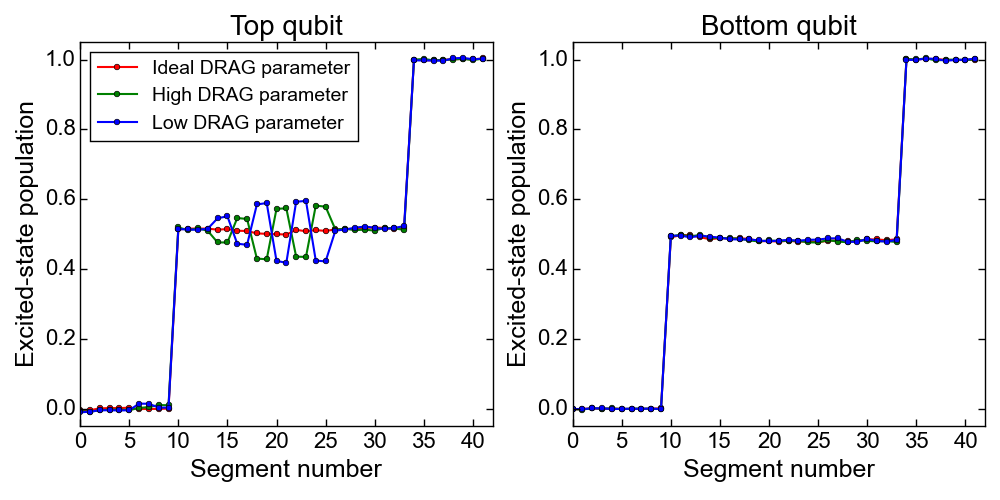
\includegraphics[width=1\linewidth]{../Figures/Exploring frequency re-use/AllXY_drag_top.png}
         \caption{}
         \label{fig:AllXY DRAG top}
      \end{subfigure}

      \caption[Two numerical solutions]{AllXY measurement of the top and bottom qubit as one parameter of the top qubit is varied. The parameter varied is (a) drive amplitude, (b) DRAG amplitude. The AllXY sequences are placed on top of each other. As can be seen the bottom qubit has no noticeable change in the AllXY measurements when the parameters of the top qubit are varied.}
      \label{fig:AllXY individual control}
      \end{figure}



    \begin{itemize}
      \item The Muxmon0 and Muxmon1 chip are designed with two purposes
      \begin{enumerate}
        \item Testing multiplexing using the Duplexer
        \item Explore qubit frequency re-use
      \end{enumerate}
    \end{itemize}

    \textbf{Ideas:}
    \begin{itemize}
      \item Title could be frequency re-use and multiplexing / selective broadcasting
    \end{itemize}

  \chapter{Exploring the Muxmon chip}
    \section{Properties of the Muxmon0 chip}

      \begin{figure}[tb]
        \centering
        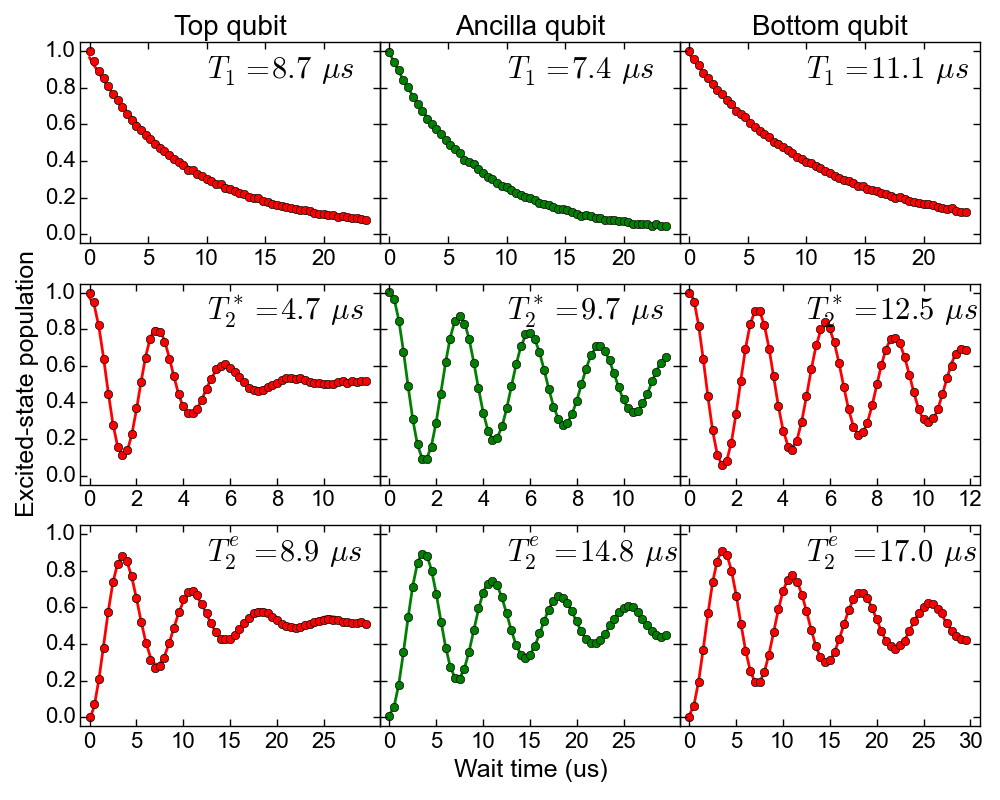
\includegraphics[width=\linewidth]{../Figures/Exploring frequency re-use/coherence_times.png}
        \caption{Coherence times of the three qubits in Muxmon0. The top qubit frequency is tuned to match the bottom qubit frequency (\SI{6.22}{\giga \hertz}).}
        \label{fig:coherence times Muxmon0}
      \end{figure}

      \begin{table}
        \begin{tabular}{l || c | c | c}
          Qubit  & $f_\text{max}$ (GHz) & $f_\text{res}$ (GHz) & coupling strength $g$ \\
          \hline
          Top    & 6.277                & 6.700                & ?\\
          Ancilla& 6.551                & 6.733                & ? \\
          Bottom & 6.220                & 6.800                & ?
        \end{tabular}
        \caption{Sweet-spot frequencies $f_\text{max}$, resonator frequencies $f_\text{res}$ and coupling strengths $g$ of the three qubits in the Muxmon0 chip}
        \label{tab:Muxmon0 qubit properties}
      \end{table}
      In the Muxmon0 chip the top and bottom qubits are each coupled to the ancilla qubit via a resonator bus. The frequencies of the qubits and their corresponding resonators are shown in Table~\ref{tab:Muxmon0 qubit properties}. All three qubits are operating in the dispersive regime, as the minimum detuning is considerably larger than the coupling strength for all qubits. The resonator buses have a frequency of \SI{4.88}{\giga \hertz} and \SI{4.97}{\giga \hertz} for the bus connecting the ancilla qubit to the top and bottom qubit respectively (see Appendix~\ref{sec:Resonator buses}. These buses can be used for multi-qubit operations, such as excitation swapping.

      To study frequency re-use, the top qubit frequency has been tuned to that of the bottom qubit, while the ancilla and bottom qubits were kept at their respective sweet-spots. Under these conditions the coherence times of the three qubits are shown in Figure~\ref{fig:coherence times Muxmon0}. The dephasing time $T_2^*$ of the top qubit is considerably worse than of the ancilla and bottom qubit. This is because the top qubit has been tuned away from its sweet-spot, and so is more susceptible to flux noise.

      \textbf{TODO:}
      \begin{itemize}
        \item explain top ancilla and bottom qubit
        \item find coupling strengths
        \item  The fit to $T_2^*$ of the top qubit has been performed using a Gaussian noise model.
      \end{itemize}


    \section{Cross-coupling}
      \label{sec:cross-coupling}
      \begin{figure}[tb]
        \centering
        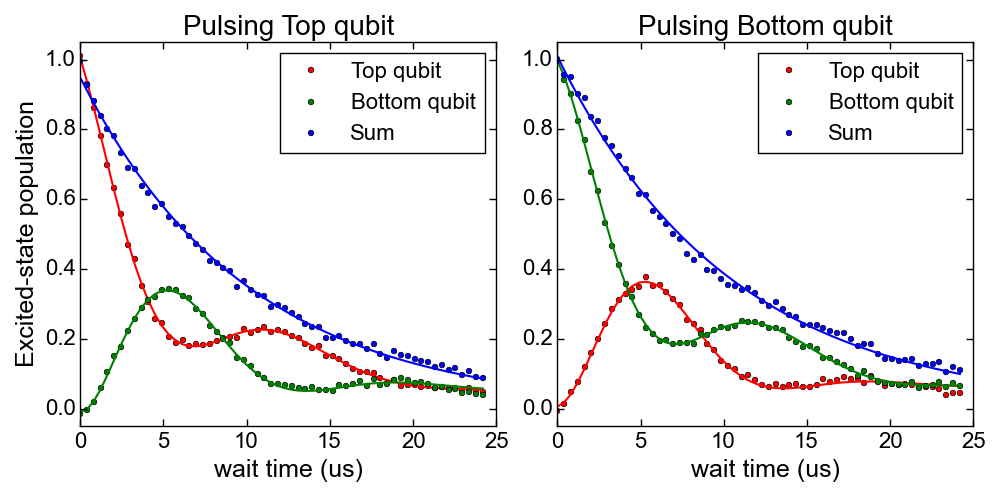
\includegraphics[width=\linewidth]{../Figures/Exploring frequency re-use/excitation_swap.png}
        \caption{After initially exciting one qubit, and measuring the excited-state population of both qubits versus time, an excitation swap is observed. The extracted coupling strength is equal to $J2\pi=72.0 \pm 1.8$ kHz}
        \label{fig:excitation swap}
      \end{figure}

      The top qubit is coupled to the botom qubit via the following three successive components:

      \begin{enumerate}
        \item The resonator bus coupling the top qubit to the ancilla qubit.
        \item The ancilla qubit.
        \item The resonator bus coupling the two ancilla qubit to the bottom qubit.
      \end{enumerate}

      When the top and bottom qubit are tuned into resonance, the two qubits experience an exchange interaction. This interaction leads to an excitation in one qubit being able to travel to the other qubit. This can result in the swapping of excitation between the top and bottom qubit, at a rate given by the interaction strength $J$. The excitation swapping of the top and bottom qubit when tuned into resonance can be seen in Figure~\ref{fig:excitation swap}. From these results the coupling $J$ is found to be equal to $J/2\pi=72. \pm 1.8$ kHz. For more information on the exchange interaction see section~4.3.2 of the thesis by Chow \cite{Chow}.

    \section{Cross-driving}
      \label{sec:cross-driving}

      \begin{figure}[tb]
        \centering
        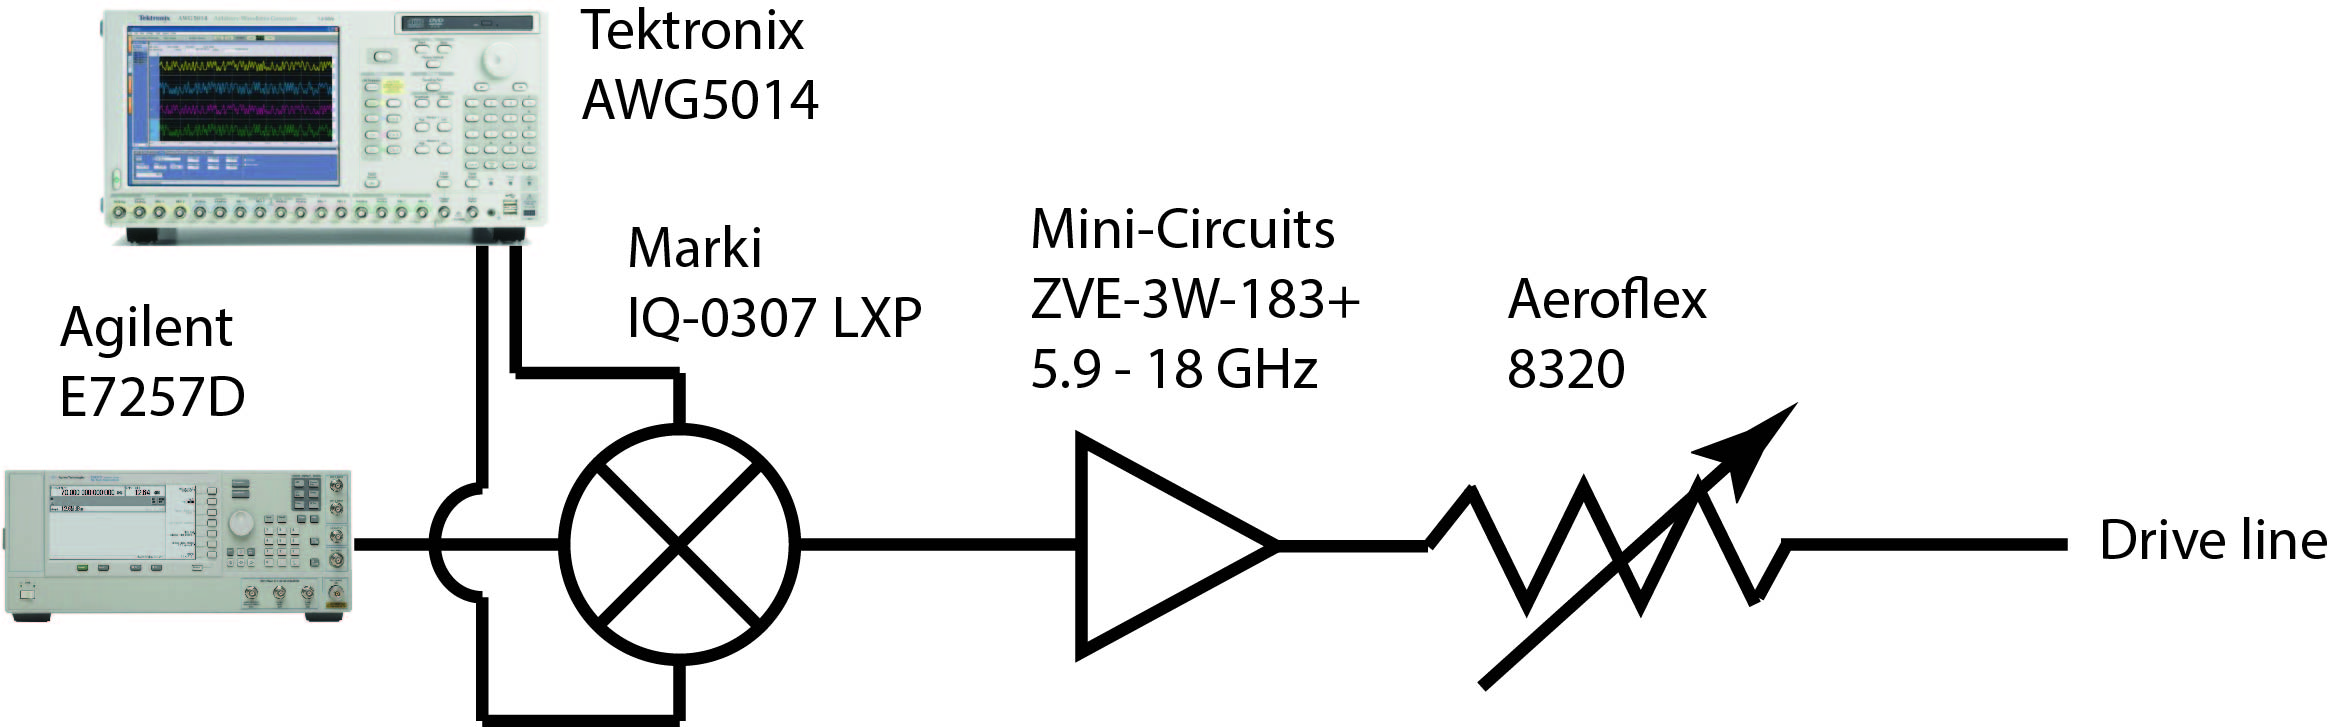
\includegraphics[width=.8\textwidth]{../Figures/Exploring frequency re-use/cross-driving_setup.jpg}
        \caption{Schematic for measuring the amount of cross-driving using the direct drive lines of the top and bottom qubit. The combination of amplifier and variable attenuator allow a range range of drive strengths.}
        \label{fig:cross-driving schematic}
      \end{figure}

      {\centering
        \begin{minipage}{0.65\textwidth}
          \centering
          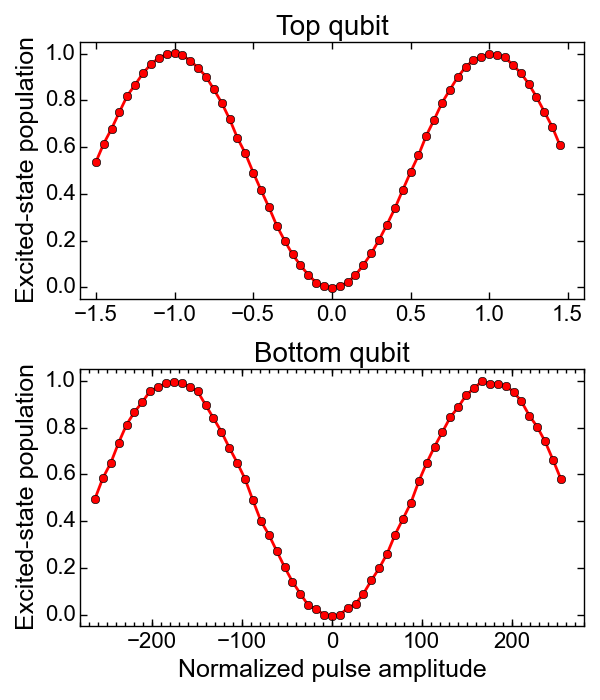
\includegraphics[width=\textwidth]{../Figures/Exploring frequency re-use/cross-driving_Rabi.png}
          \captionof{figure}{Required drive amplitude required to drive the top and bottom qubit through the top qubit drive line. The amplitude has been normalize to the amplitude required for a pi pulse on the top qubit.}
          \label{fig:cross-driving Rabi}
        \end{minipage}
        \begin{minipage}{0.35\textwidth}
          \centering
          \begin{tabular}{c | c}
            qubit & cross-driving (\%) \\
            \hline
            Top & $-$ \\
            Ancilla &$ 0.79$ \\
            Bottom & $0.57$
          \label{tab:cross-driving top}
          \end{tabular}
          \captionof{table}{Driving through top qubit drive line}
          \vspace{2cm}
          \begin{tabular}{c | c}
            qubit & cross-driving (\%) \\
            \hline
            Top & $0.23$ \\
            Ancilla &$ 0.66$ \\
            Bottom & $-$
          \end{tabular}
          \captionof{table}{Driving through bottom qubit drive line}
          \label{tab:cross-driving bottom}
        \end{minipage}
      \vspace{1cm}
      }

      When driving one of the qubits through its dedicated drive line, the signal can partially leak through to the other qubits. The cause of this leakage may be on-chip, where the components separating the qubits do not fully filter the signal, or may be off-chip, due to for instance imperfect isolation between the cables or other components. This signal leakage results in cross-driving effect, where driving one qubit will also partially drive the other qubits. Cross-driving effects affect the performance of the qubits when the frequency of the driven qubit and the cross-driven qubit are in resonance, as is the case with the Muxmon experiment.

      The amount of cross-driving can be determined by measuring the pulse amplitude required to drive each of the three qubits through a drive line. The cross-driving due to the finite isolation of the Duplexer has been separately measured (see Appendix~\ref{ch:Duplexer isolation}). At the frequencies used in the experiment, the isolation of the Duplexer was found to be typically around \SI{50}{\dBm}. The amount of cross-driving due to other sources was determined by measuring the pulse amplitude required to perform a Rabi on each of the qubits using a fixed drive line. The measurements were performed using the set-up shown in Figure~\ref{fig:cross-driving schematic}. The results of a single cross-driving measurement is shown in Figure~\ref{fig:cross-driving Rabi}, where the top and bottom qubit are driven through the drive line of the top qubit. The pulse amplitude is normalized to the amplitude required for applying pi pulse to the qubit directly connected to the drive line. The amount of cross-driving is equal to the ratio of the pulse amplitude required for a pi rotation for the main qubit, and for the cross-driven qubit. The cross-driving ratio's are shown in Tables~\ref{tab:cross-driving top} and ~\ref{tab:cross-driving bottom}. The cross-driving ratio's are found to be less than one percent, and are higher for the ancilla qubit than for the other cross-driven qubit. This indicates that the main source of cross-driving is likely on-chip. Furthermore it can be seen that the cross-driving is stronger from the drive line of the top qubit than from the drive line of the bottom qubit.

      \begin{wrapfigure}[12]{r}{0.45\textwidth}
        \begin{center}
        \vspace{-30pt}
          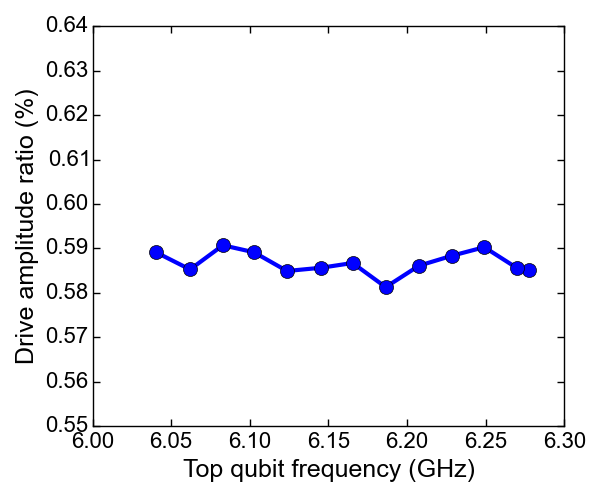
\includegraphics[width=\textwidth]{../Figures/Exploring frequency re-use/cross-driving_vs_top_frequency.png}
        \end{center}
        \vspace{-20 pt}
        \caption{Cross-driving ratio of the bottom qubit when pulsing from the drive line of the top qubit, versus frequency of the top qubit. }
        \label{fig:cross-driving versus top frequency}
      \end{wrapfigure}

      As a check that the effects observed are indeed due to cross-driving, and not due to cross-coupling, the cross-driving when driving the bottom qubit through the drive line of the top qubit has been measured as the frequency of the top qubit is varied. The results are shown in Figure~\ref{fig:cross-driving versus top frequency}. If the effect is due to cross-coupling the amount of cross-driving should depend strongly on the detuning between the top qubit and bottom qubit. Instead we see that the cross-driving is approximately constant, indicating that this is indeed a cross-driving effect instead of a cross-coupling effect.


    \textbf{Figures that need to be included:}
    \begin{itemize}
      \item schematic of cross-coupling and readout cross-talk \\
          It could be good to create this using the actual Muxmon chip as background, with arrows indicating how the different effects operate
    \end{itemize}


  \chapter{Randomized benchmarking}
    \label{ch:randomized benchmarking}

    \section{Introduction}
      \label{sec:RB introduction}
      When preparing the qubits for a quantum algorithm it is important to know what the performance is of the qubits, which can be characterized by its gate errors. One method has already been discussed in Section~\ref{sec:AllXY}, namely the AllXY method. Although the AllXY is good at detecting specific errors, it is a crude method, which is unable to characterize gate errors with high accuracy. Another method used for gate characterization is quantum process tomography. Quantum process tomography measures the output density matrix resulting from the application of a specific to each of the system's basis states. Due to linear superposition of quantum states, the full effect of a gate is thereby characterized.

      Quantum process tomography suffers from some important drawbacks. The first is that it is sensitive to state preparation and measurement errors, which make it difficult to distinguish whether the gate errors originate from the actual gate being characterized, or from the gates used for preparation and measurement. Another related drawback is that it is unable to measure small gate errors, which are required for fault-tolerant quantum computing. Additionally, quantum process tomography suffers from an exponential scaling in measurement with the number of qubits. These drawbacks result in quantum process tomography being an inadequate gate characterization method for gates with small errors.

      An alternative method to quantum process tomography is randomized benchmarking. It is based on repeated application of gates drawn randomly from a set of unitary operations, after which the fidelity to the final state in absence of errors is measured. The set of unitaries used in randomized benchmarking may be single-qubit or multi-qubit operations. Randomized benchmarking has the advantage that it is insensitive to state preparation and measurement errors, and is a relatively fast measurement, which is able to accurately determine the average unitary operation error.

      In the Muxmon experiment the set of unitary operations is the single-qubit Clifford group, which will be discussed in Section~\ref{sec:Clifford group}. Randomized benchmarking will be used to characterize the performance of the qubits when using the Duplexer, and using selective broadcasting. By interleaving the unitary operations with a fixed gate the performance of that specific gate can be measured. This is known as interleaved randomized benchmarking, and will be discussed in Section~\ref{sec:interleaved randomized benchmarking}.

      \begin{itemize}
        \item uniform sampling on bloch sphere
        \item Process tomography shows the type of error
      \end{itemize}

    \section{Clifford group}
      \label{sec:Clifford group}

      \begin{figure}[h]%[12]{r}{0.45\textwidth}
        \begin{center}
          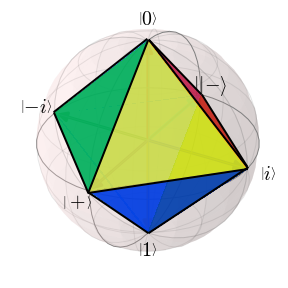
\includegraphics[width=.5\textwidth]{../Figures/Randomized benchmarking/Bloch sphere octahedron.png}
        \end{center}
        \caption{The single-qubit Clifford group can be visualized using an octahedron whose vertices correspond to the six cardinal states. The 24 Cliffords composing the single-qubit Clifford group correspond to the 24 distinct rotations of the octahedron such that the vertices are mapped onto themselves.}
        \label{fig:Clifford octahedron}
      \end{figure}

      The single qubit Pauli group consists of the two-dimensional identity operator and the three Pauli matrices. The $n$ qubit Pauli group is generated by the tensor product of $n$ single qubit Pauli groups. The $n$ qubit Clifford group $\mathpzc{C}_n$ is equal to the set of unitary transformations on the $n$ qubit Pauli group up to a global phase. The $n$ qubit Clifford group $\mathpzc{C}_n$ is generated by $\{H_i, P_i, CNOT_{ij}\} \forall i, j \in (1, \dots, n)$, where:

      \begin{equation}
        H =
        \frac{1}{\sqrt{2}}
        \begin{pmatrix}
          1 & 1 \\
          1 & 1
        \end{pmatrix}, \qquad
        P =
        \frac{1}{\sqrt{2}}
        \begin{pmatrix}
          1 & 0 \\
          0 & i
        \end{pmatrix}, \qquad
        CNOT =
        \frac{1}{\sqrt{2}}
        \begin{pmatrix}
          1 & 0 & 0 & 0 \\
          0 & 1 & 0 & 0 \\
          0 & 0 & 0 & 1 \\
          0 & 0 & 1 & 0
        \end{pmatrix}
      \end{equation}

      The single qubit Clifford group $\mathpzc{C}_1$ can be visualized using an octahedron in the Bloch sphere, as shown in Figure~\ref{fig:Clifford octahedron}. Each Clifford in $\mathpzc{C}_1$ corresponds to a distinct rotation of the octahedron, where the six cardinal states are mapped onto themselves. If one sets the constraint that the state $\ket{0}$ is mapped to itself, four distinct rotations are possible. Since the state $\ket{0}$ can be mapped to each of the six cardinal states, there are $6 \times 4=24$ distinct rotations, and hence $24$ Cliffords in the single qubit Clifford group $\mathpzc{C}_1$.

      Each of the Cliffords in the single qubit Clifford group $\mathpzc{C}_1$ can be decomposed into rotations along the X and Y axis, as is shown in Appendix~\ref{ssec:Clifford gate decomposition}. Each Clifford can be decomposed into a minimum of zero (identity) gates and a maximum of three gates. If one includes the identity as a gate, a Clifford requires on average 1.875 gates.

      The Clifford group does not form a universal set of gates. This is because the rotations only map cardinal states onto themselves. Since single qubit gates and CNOT is universal (\cite{nielsen2010quantum}), the Clifford group combined with the T-gate ($\pi/4$ rotation) constitute a set of universal quantum gates.

    \section{The randomized benchmarking protocol}
      \label{sec:randomized benchmarking protocol}

      \begin{wrapfigure}[7]{r}{0.4\textwidth}
        \begin{center}
        \vspace{-30pt}
          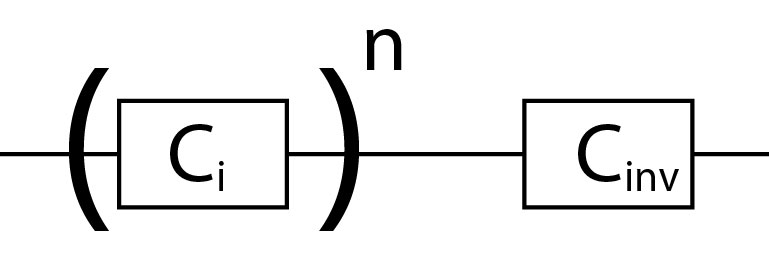
\includegraphics[width=.8\textwidth]{../Figures/Randomized benchmarking/RB schematic.jpg}
        \end{center}
        \vspace{-20 pt}
        \caption{Schematic of the randomized benchmarking protocol}
        \label{fig:RB schematic}
      \end{wrapfigure}

      Randomized benchmarking is a method to characterize the performance on qubits. It is based on repeated application of operations on the system, and measuring the fidelity to the ideal final state. The operations are randomly chosen from a set of unitary operations.

      In the case of the Muxmon experiment randomized benchmarking is performed on individual qubits, and the set of unitary operations is the single qubit Clifford group. The randomized benchmarking protocol used in this experiment, depicted in Figure~\ref{fig:RB schematic}, is as follows:

      \begin{enumerate}
        \item Initialize the qubit in the ground state
        \item Apply $n$ consecutive Cliffords $\{C_1, \dots, C_n\}$, where $C_i \in \mathpzc{C}_1 \; \forall \; i \in \left[1, \dots, n\right]$
        \item apply final inverting Clifford $C_\text{inv}=\left( C_n \dots C_1 \right)^{-1}$
        \item Measure the state of the qubit
      \end{enumerate}

      After the final inverting Clifford $C_\text{inv}$ the qubit should return to the ground-state. However, gate errors and decoherence result in the final state deviating from the ground-state. The qubit will therefore be in the excited-state with a nonzero probability. This probability increases as the number of Cliffords $n$ is increased.

      \textbf{TODO:} Something about exponential decay
      \begin{equation}
        P= A p^n + B
        \label{eq:RB exponential decay}
      \end{equation}

      \begin{figure}[tb]
        \centering
        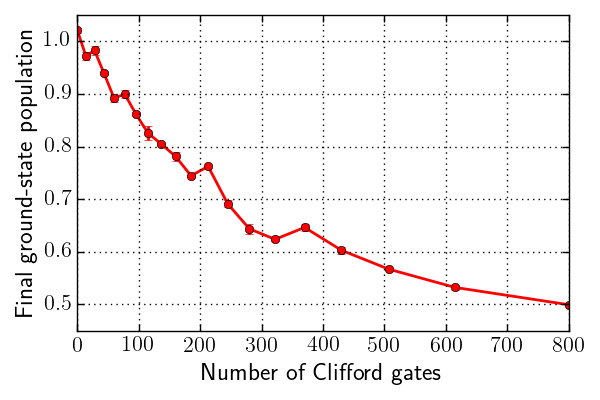
\includegraphics[width=.6\textwidth]{../Figures/Randomized benchmarking/RB_single_seed.png}
        \caption{Randomized benchmarking results using a single seed. The final ground-state population decreases exponentially as the number of Cliffords $n$ is increased. The points include errorbars, determined by the spread of three separate measurements.}
        \label{fig:RB single seed}
      \end{figure}

      To characterize the shape of the exponential decay, the successive values of $n$ in a measurement are separated by an exponentially increasing amount. The randomized benchmarking results using a single seed are shown in Figure~\ref{fig:RB single seed}. Twenty points are chosen between $n=0$ and $n=800$ Clifford operations. As can be seen there is a clear exponential decay, in agreement with Formula~\ref{eq:RB exponential decay}. However, upon closer inspection the curve does not have a perfect exponential shape. This deviation is not due to insufficient averaging, but due to the fact that the Cliffords do not all have the same number of gates. A Clifford is on average composed of $1.875$ gates, but may be composed of anywhere between $1$ and $3$ gates. The result is that in a single seed some segments contain on average more than $1.875$ gates per Clifford, while other contain less. For a fixed error per gate, this results in fidelities deviating from the fidelity corresponding to exactly $1.875$ gates per Clifford. To obtain an accurate estimate for the exponential decay rate, multiple seeds must be used to average out the random fluctuations from the average gate per Clifford.

      \begin{itemize}
        \item Clifford group can be efficiently simulated on a classical computer. Gottesman-Knill theorem (\cite{gottesman1998heisenberg})
        \item Explain the formula relating $n$ to an exponential curve.
        \item Coherence limit of RB
      \end{itemize}

    \section{Driving a single qubit versus driving both qubits}
      \label{sec:Driving a single qubit versus driving both qubits}



      \begin{figure}[tb]
        \centering
        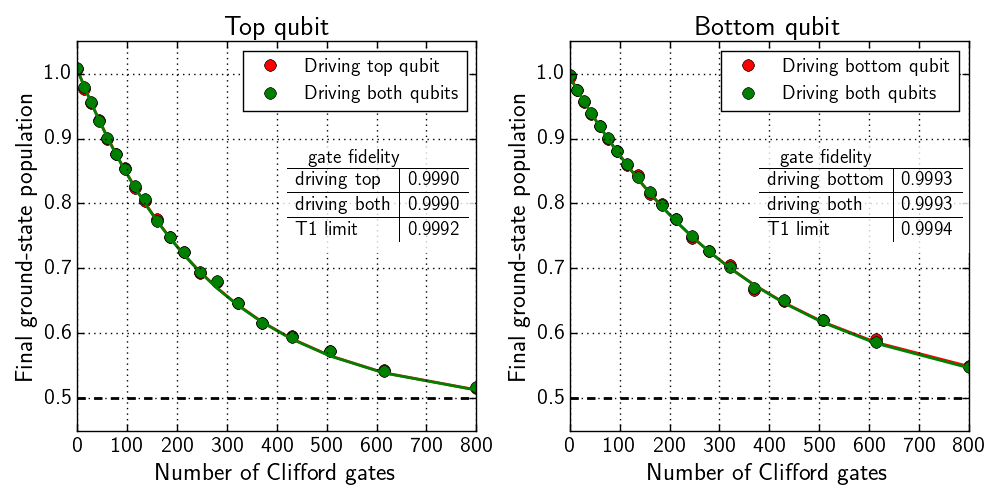
\includegraphics[width=\textwidth]{../Figures/Randomized benchmarking/RB_normal_driving_single_both.png}
        \caption{Randomized benchmarking results when driving a single qubit versus driving both qubits simultaneously. As can be seen there is no noticeable difference between driving only one qubit versus driving both qubits simultaneously. A total of 50 different seeds were used.}
        \label{fig:RB normal single vs both}
      \end{figure}


      \begin{figure}[tb]
        \centering
        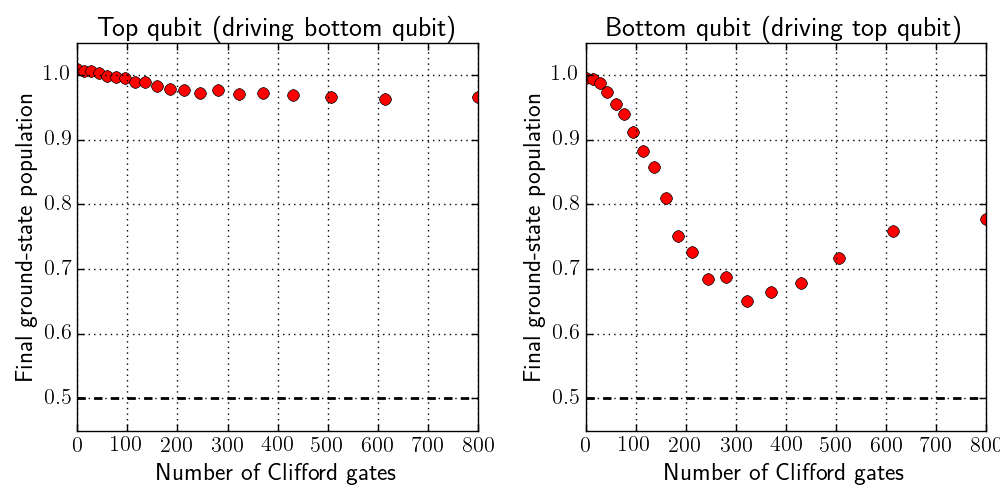
\includegraphics[width=\textwidth]{../Figures/Randomized benchmarking/RB_normal_cross-driving.png}
        \caption{Excitation in qubit when only the other qubit is driven during randomized benchmarking. This effect is mostly due to cross-driving and is considerably stronger for the top qubit than for the bottom qubit.}
        \label{fig:RB normal cross-driving}
      \end{figure}

      \begin{figure}[tb]
        \centering
        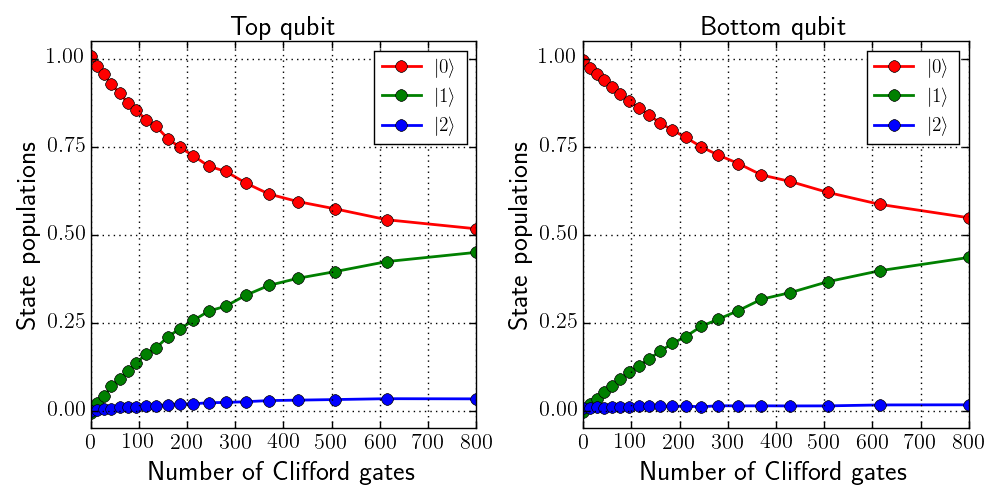
\includegraphics[width=\textwidth]{../Figures/Randomized benchmarking/RB_normal_state_populations.png}
        \caption{Caption here}
        \label{fig:RB normal state populations}
      \end{figure}


    \section{Interleaved randomized benchmarking}
      \label{sec:interleaved randomized benchmarking}

    \section{Second excited state}

  \chapter{Conclusions and outlook}
